%%%%%%%%%%%%%%%%%%%%%%%%%%%%%%%%%%%%%%%%%%%%%%%%%%%%%%%%%%%%%%%%%%%%%%%%%
%                                                                       %
% ustthesis_test.tex: A template file for usage with ustthesis.cls      %
%                                                                       %
%%%%%%%%%%%%%%%%%%%%%%%%%%%%%%%%%%%%%%%%%%%%%%%%%%%%%%%%%%%%%%%%%%%%%%%%%

\documentclass{ustthesis}
\usepackage{mathpazo,amsmath,amssymb,epsfig,enumerate,bbm,calc,color,ifthen,capt-of} % original was times, but I think it's ugly; we use the same as IEEE CompSoc
\usepackage{algorithm}
\usepackage{url}
\usepackage{booktabs}
\usepackage{slashbox}
\usepackage{float}
\usepackage{commath}
\usepackage{tabularx}
\usepackage{epsf}
\usepackage[noend]{algorithmic}
\usepackage[center]{subfigure}
\usepackage{listings}
\lstset{breaklines}
\lstset{extendedchars=false}
\usepackage{wrapfig}
\usepackage{color,graphicx}
\usepackage[export]{adjustbox}
\newtheorem{proof}{Proof}
\usepackage{hyperref} % for better viewing experience  -- added by alan
\usepackage[margin=25mm,textheight=247mm,textwidth=145mm]{geometry}

% Alan: begin the font trial
% Euler for math | Palatino for rm | Helvetica for ss | Courier for tt
\renewcommand{\rmdefault}{ppl} % rm
%\linespread{1.05}        % Palatino needs more leading
\usepackage[scaled]{helvet} % ss
\usepackage{courier} % tt 
\usepackage{eulervm} % a better implementation of the euler package (not in gwTeX)
\normalfont
\usepackage[T1]{fontenc}
% Alan: end the font trial

\newcommand{\red}[1]{#1}
\newcommand{\tab}[1]{\hspace{3mm}}

% \usepackage{latexsym}
    % Use the "latexsym" package when encountering the following error:
    %   ! LaTeX Error: Command \??? not provided in base LaTeX2e.
% \usepackage{epsf}
    % Use the "epsf" package for including EPS files.

%%%%%%%%%%%%%%%%%%%%%%%%%%%%%%%%%%%%%%%%%%%%%%%%%%%%%%%%%%%%%%%%%%%%%%%%%
%                                                                       %
% Preambles. DO NOT ERASE THEM. Change to suite your particular purpose.%
%                                                                       %
%%%%%%%%%%%%%%%%%%%%%%%%%%%%%%%%%%%%%%%%%%%%%%%%%%%%%%%%%%%%%%%%%%%%%%%%%

\title{Electrodynamic Tether Satellite Dynamics Modelling}  % Title of the thesis.
\author{Kaiwen~Chen}     % Author of the thesis.
\degree{\MSc}             % Degree for which the thesis is.
\subject{Aeronautical Engineering}      % Subject of the Degree.
\department{Mechanical and Aerospace Engineering}       % Department to which the thesis
                    % is submitted.
\advisor{Prof.~Xun~HUANG}     % Supervisor.
    
\defencedate{2018}{05}{29}      % \defencedate{year}{month}{day}.

% NOTE:
%   According to the sample shown in the guidelines, page number is
%   placed below the bottom margin.  However, if the author prefers
%   the page number to be printed above the bottom margin, please
%   activate the following command.

% \PNumberAboveBottomMargin

\begin{document}

%%%%%%%%%%%%%%%%%%%%%%%%%%%%%%%%%%%%%%%%%%%%%%%%%%%%%%%%%%%%%%%%%%%%%%%%%
%                                                                       %
% Now the actual Thesis. The order of output MUST be followed:          %
%                                                                       %
%    1) TITLEPAGE                                                       %
%                                                                       %
% The \maketitle command generates the Title page as well as the        %
% Signature page.                                                       %
%                                                                       %
%%%%%%%%%%%%%%%%%%%%%%%%%%%%%%%%%%%%%%%%%%%%%%%%%%%%%%%%%%%%%%%%%%%%%%%%%

\maketitle

%%%%%%%%%%%%%%%%%%%%%%%%%%%%%%%%%%%%%%%%%%%%%%%%%%%%%%%%%%%%%%%%%%%%%%%%%
%                                                                       %
%     2) DEDICATION (Optional)                                          %
%                                                                       %
% The \dedication and \enddedication commands are optional. If          %
% specified it generates a page for dedication.                         %
%
%%%%%%%%%%%%%%%%%%%%%%%%%%%%%%%%%%%%%%%%%%%%%%%%%%%%%%%%%%%%%%%%%%%%%%%%%

% \dedication
% This is an optional section.
% \enddedication

%%%%%%%%%%%%%%%%%%%%%%%%%%%%%%%%%%%%%%%%%%%%%%%%%%%%%%%%%%%%%%%%%%%%%%%%%
%                                                                       %
%     3) ACKNOWLEDGMENTS                                                %
%                                                                       %
% \acknowledgments and \endacknowledgments defines the                  %
% Acknowledgments of the author of the Thesis.                          %
%                                                                       %
%%%%%%%%%%%%%%%%%%%%%%%%%%%%%%%%%%%%%%%%%%%%%%%%%%%%%%%%%%%%%%%%%%%%%%%%%

\acknowledgments
I would never have completed this work without the help from many people. First of all, I thank my advisor, Professor Xun Huang, for his kind mentoring, helpful advices, and encouragement. I have got generous material support, well-condition laboratory experiences and engineering-oriented practice.  

I thank the members of my thesis committee, Professor Xin Zhang for his insightful comments on improving this work. 

I thank my colleagues in HKUST -- Huanxian Bu, Zheng Liu, Wei Feng, Jiafeng Wu, Jingwen Guo, Jiaqi Song and many others. We have finished several deadlines and projects as a team. In daily life, we have been good friends and enjoy many activities in school campus. Without them, my graduate study in HKUST would not be so colorful. 

I give my special thanks to Dr.Pok Wang KWAN who spent nearly a whole year instructing me on how to do research. He gave the project a lot of remarkable ideas using his sufficient engineering background and rich industry experience. When everything goes more and more complicated, his clear mind and intuition always work quite well. I learned how to proceed an engineering research project and how to analyse problems logically and incrementally from his face to face teaching.

I thank Github user Cheedoong and wenbinf for their contribution and sharing of the HKUST Latex thesis Template. This thesis is writing in Latex based on that template-ustthesis Latex class. It saves me a lot of time to do typesetting and let me focus on the contents.   

I thank my parents for their support and encouragement. 

Hope this thesis will not be the end of my academia, I hope the first half sentence is not just a hope.

\endacknowledgments

%%%%%%%%%%%%%%%%%%%%%%%%%%%%%%%%%%%%%%%%%%%%%%%%%%%%%%%%%%%%%%%%%%%%%%%%%
%                                                                       %
%     4) TABLE OF CONTENTS                                              %
%                                                                       %
%%%%%%%%%%%%%%%%%%%%%%%%%%%%%%%%%%%%%%%%%%%%%%%%%%%%%%%%%%%%%%%%%%%%%%%%%

\tableofcontents

%%%%%%%%%%%%%%%%%%%%%%%%%%%%%%%%%%%%%%%%%%%%%%%%%%%%%%%%%%%%%%%%%%%%%%%%%
%                                                                       %
%     5) LIST OF FIGURES (If Any)                                       %
%                                                                       %
%%%%%%%%%%%%%%%%%%%%%%%%%%%%%%%%%%%%%%%%%%%%%%%%%%%%%%%%%%%%%%%%%%%%%%%%%

\listoffigures

%%%%%%%%%%%%%%%%%%%%%%%%%%%%%%%%%%%%%%%%%%%%%%%%%%%%%%%%%%%%%%%%%%%%%%%%%
%                                                                       %
%     6) LIST OF TABLES (If Any)
%                                                                       %
%%%%%%%%%%%%%%%%%%%%%%%%%%%%%%%%%%%%%%%%%%%%%%%%%%%%%%%%%%%%%%%%%%%%%%%%%

\listoftables

%%%%%%%%%%%%%%%%%%%%%%%%%%%%%%%%%%%%%%%%%%%%%%%%%%%%%%%%%%%%%%%%%%%%%%%%%
%                                                                       %
%     7) ABSTRACT                                                       %
%                                                                       %
% \abstract and \endabstract are used to define a short Abstract for    %
% the Thesis.                                                           %
%                                                                       %
%%%%%%%%%%%%%%%%%%%%%%%%%%%%%%%%%%%%%%%%%%%%%%%%%%%%%%%%%%%%%%%%%%%%%%%%%

\begin{abstract}
Abstract
\end{abstract}


%%%%%%%%%%%%%%%%%%%%%%%%%%%%%%%%%%%%%%%%%%%%%%%%%%%%%%%%%%%%%%%%%%%%%%%%%
%                                                                       %
%     8) The Actual Contents                                            %
%                                                                       %
% The command \chapters MUST BE USED to ensure that the entire content  %
% of the Thesis is double-spaced (in version 1.0).                      %
%                                                                       %
% However, in version 2.0, \chapters will be automatically added in     %
% the beginning of the first chapter.                                   %
%                                                                       %
%%%%%%%%%%%%%%%%%%%%%%%%%%%%%%%%%%%%%%%%%%%%%%%%%%%%%%%%%%%%%%%%%%%%%%%%%

%%\chapters         % Not necessary with ustthesis.cls (v2.0).

%%%%%%%%%%%%%%%%%%%%%%%%%%%%%%%%%%%%%%%%%%%%%%%%%%%%%%%%%%%%%%%%%%%%%%%%%
%                                                                       %
% Each chapter is defined via the \chapter command. The usual sectional %
% commands of LaTeX are also available.                                 %
%                                                                       %
%%%%%%%%%%%%%%%%%%%%%%%%%%%%%%%%%%%%%%%%%%%%%%%%%%%%%%%%%%%%%%%%%%%%%%%%%

\input{chapter/section-Motivation}
\chapter{Literature Review}\label{sec-literature}
\section{Space tether past missions}
\begin{enumerate} 


\item{NASA}
 
NASA has been developing tether technology for space applications since the 1960s, including electrodynamic tether propulsion, the Propulsive Small Expendable Deployer System (ProSEDS) flight experiment, ” Hanging” momentum exchange tethers, rotating momentum exchange tethers and tethers supporting scientific space research. 

\item{NASA-Gemini XI} 

The Gemini XI was a manned spaceflight in NASA’s Gemini program, launched on September 12,1966. One of the main objectives was related to tethers. It was synoptic terrain photography and a tethered vehicle test. The objectives were all achieved. 

\item{NASA-Gemini XII} 
   
The Gemini XII was a manned spaceflight in NASA’s Gemini program launched on November 11, 1966. One of its major objectives was tethered vehicle evaluation. The objective was achieved.
\item{Tethered Payload Experiment (TPE)}

TPE-1mission was launched on January 16, 1980. Its plan was to deploy 400 metres of cable, but its deployed cable was about 38 metres. The TPE-2 mission was launched on 29 January, 1981, and its tether was deployed to a distance about 65 metres. In 1983, the TPE-3, which was also called CHARGE-1, had a length of about 500m. As the deployment system was improved, the tether deployed to its full length of 418 meters, and the tether was also found to act as a radio antenna for the electrical current through the cable. CHARGE-2 was carried out as an international program between Japan and the USA using a NASA sounding rocket at White Sands Missile Range, in December 1985, its tether deployed to a length of 426 metres.
CHARGE-2B tethered rocket mission was launched in 1992 by NASA with a Black Brant V rocket. The mission was to generate electromagnetic waves by modulating the electron beam. The tether was fully deployed over 400 meters and the experiments all worked as planned.
\item{NASA and NDRE-MAIMIK}

	The tether length of MAIMIK was about 400m. The mission was designed to study the charging of an electron-beam emitting payload using a tethered mother-daughter payload configuration. 

\item{US Air Force Geophysics Lab- Echo-7}

Designed to study the artificial electron beam propagation along magnetic field lines in space, the mission planned to study how the artificial electron beam propagates along magnetic field lines in space.
\item{OEDIPUS}

OEDIPUS-A. The conducting tether was deployed over 985 metres during the flight of a Black Brant sounding rocket in to the auroral ionosphere.
OEDIPUS-C. The following OEDIPUS mission was the OEDIPUS-C tethered payload mission, which was launched in 1995 with an 1174-metre deployed tether, and a Tether Dynamics Experiment (TDE) was also included as a part of the OEDIPUS-C.
\item{Tethered Satellite System (TSS)}

The first orbital flight experiment with a long tether was the Tethered Satellite System (TSS) mission, launched on the Space Shuttle in July 1992. The Tethered Satellite System-1 (TSS-1) was flown during STS-46, aboard the Space Shuttle Atlantis, from July 31 to August 8, 1992. The TSS-1 mission discovered a lot about the dynamics of the tethered system. Although the satellite was deployed only 260 metres, it was able to show that the tether could be deployed, controlled, and retrieved, and that the TSS was easy to control, and even more stable than predicted. The TSS was an electrodynamic tether, its deployment mechanism jammed resulting in tether sever and less than 1000 metres of deployment. The objectives of TSS-1 were (1) to verify the performance of the TSS equipment; (2) to study the electromagnetic interaction between the tether and the ambient space plasma; (3) to investigate the dynamical forces acting on a tethered satellite. In the first tether deployment, when the satellite was moving excessively from side to side, the deployment was aborted. The second trial of deployment was unreeled to a length of 260 metres.
In 1996, the Tethered Satellite System Reflight (TSS-1R) was carried by using US space shuttle STS-75 successfully. The primary objective of STS-75 was to carry the Tethered Satellite System Reflight (TSS-1R) into orbit and to deploy it spacewards on a conducting tether.
\item{Shuttle Electrodynamic Tether System (SETS)}

	The Shuttle Electrodynamic Tether System (SETS) experiment formed part of the scientific experiments comprising the first flight of the NASA/ASI Tethered-Satellite System flown at an altitude of 300 km and at an orbital inclination of 28.5 degrees in July/August 1992. The SETS experiment was designed to study the electrodynamic behaviour of the Orbiter-Tether-Satellite system, as well as to provide background measurements of the ionospheric environment near the Orbiter. The SETS experiment was able to operate continuously during the mission thereby providing a large data set.
\item{Small Expendable Deployer System (SEDS)}

The Small Expendable Deployer System-1 (SEDS-1) was launched from Cape Canaveral Air Force Station as a Delta/GPS secondary payload in 1993. SEDS-1 was the first successful 20-kilometre space-tether experiment. When 1 km of tether remained, active braking was applied by wrapping the tether around a “barber pole” brake. Finally, the braking system and sensors did not work as predicted, resulting in hard stop/endmass recoil at deployment completion.
The Small Expendable Deployer System-2 (SEDS-2) was launched on the last GPS Block 2 satellite in 1994. The SEDS-2 used feedback braking, which was started early in deployment. This limited the residual swing after deployment to 4 degrees. Mission success was defined as deployment of at least 18 km, plus a residual swing angle of less than 15 degrees. The SEDS-2 had an improved braking system compared to SEDS-1, which was a feedback control system and applied braking force as a function of the measured speed of the unrolling tether. This was to ensure that the satellite stopped flying out just when the whole tether was deployed and to prevent the bounces experienced during the previous mission.
\item{Plasma Motor Generator (PMG)}

In 1996, the Plasma Motor Generator (PMG) was launched by NASA. This was an electrodynamic tether, which could assess the effectiveness of using hollow cathode assemblies to deploy an ionised gas, and to “ground” electrical currents by discharging the energy to space. An early experiment used a 500 metre conducting tether. When the tether was fully deployed during this test, it generated a potential of 3,500 volts. This conducting single-line tether was severed after five hours of deployment. It was believed that the failure was caused by an electric arc generated by the conductive tether’s movement through the Earth’s magnetic field. The PMG flight demonstration proved the ability of the proposed Space Station plasma grounding techniques in maintaining the electrostatic potential between the Space Station and the surrounding plasma medium, the ability to use electrostatic tethers to provide thrust to offset drag in LEO space systems and the use of direct magnetic (nonrocket) propulsion for orbital maneuvering.
\item{Tether Physics and Survivability Experiment (TiPS)}

The Tether Physics and Survivability Experiment (TiPS) was deployed on June 20, 1996 at an altitude of 1,022 kilometres as a project of the US Naval Research Laboratory. The satellite was a tether physics experiment consisting of two end masses connected by a 4 km nonconducting tether. This experiment was designed to increase knowledge about gravity-gradient tether dynamics and the survivability of tethers in space.

\item{The Young Engineers's Satellite (YES)}

The first Young Engineers’ Satellite (YES-1) programme was completed on November 3, 1997. It was designed to operate with a 35 km tether deployment, but the mission was cancelled before the flight when the launch authority changed the nominal Ariane orbit. In the new orbit configuration, a deployed 35 km tether would have constituted a hazard to the satellites in LEO.
The second Young Engineers Satellite (YES2) was launched on September 14, 2007. It was a technology demonstration project designed to test and produce data for the “Space Mail” concept, wherein a tether was used to return material from space to Earth, instead of by conventional chemical
propulsion. YES2 aimed to demonstrate a tether-assisted reentry concept, whereby the payload would be returned to Earth using momentum provided from a swinging tether. Deployment was intended to take place in two phases: (1) deployment of 3.5 km of tether to the local vertical and hold and (2) deployment to 30 km for a swinging cut. The measured altitude gain of the Fonton-M3 corresponded with what simulations showed would have happened if 31.7 km of tether were extended, another strong indication that the YES- 2 tether had in fact been fully depolyed.
The YES-2 mission was very nearly a complete success because of the following: (1) the entire record-breaking length of tether has been deployed; (2) Fotino rocket seemed to have been deorbited by using momentum exchange; (3) plentiful data has been gathered on tether deployment, dynamics and deorbiting, which may lead to an operational way of returning capsules without any form of propulsion

\item{The Advanced Tether Experiment (ATEx)}

The Advanced Tether Experiment (ATEx) was launched into orbit aboard the National Reconnaissance Office (NRO) sponsored by Space Technology Experiment spacecraft (STEX) on October 3, 1998. ATEx was intended to demonstrate the deployment and survivability of a novel tether design, as well as being used for controlled libration maneuvers. On January 16, 1999, after a deployment of only 22m of tether, ATEx was jettisoned from STEX due to an out-of-limit condition sent by the experiment’s tether angle sensor. The ATEx lower end mass was jettisoned from the host spacecraft and the tethered upper and lower end masses freely orbited the Earth in a demonstration of long-term tether survivability. 
\item{The PICOSAT mission}

The PICOSAT mission was launched on September 30, 2001. It was a real-time tracking satellite of the miniaturized picosatellite satellite series. The name “PICO” combined the first letters of all the four of its experiments, which were the Polymer Battery Experiment (PBEX), the Ionospheric Occultation Experiment (IOX), the Coherent Electromagnetic Radio Tomography (CERTO), and the On Orbit Mission Control (OOMC). A pair of 0.25kg MEMS picosatellites with an intersatellite communications experiment were included in this mission and were connected by a 30 metre tether.
\item{Propulsive Small Expendable Deployer System (ProSEDS)--\em{Cancelled}}
	
The Propulsive Small Expendable Deployer System (ProSEDS) was a NASA space tether propulsion experiment intended to be a follow up to SEDS. It was originally intended to be flown along with a launch of a Global Positioning System (GPS) satellite in the spring of 2003, but was cancelled at the last moment, due to concerns that the tether might collide with the international space station.

\item{Multi-Application Survivable Tether (MAST)}

The Multi-Application Survivable Tether (MAST) experiment was launched into LEO on April 17, 2007, in which the 1 km multistrand interconnected tether (Hoytether) was intended to test and prove the long-term survivability of tethers in space, but the tether failed to deploy. 
\item{Tether Technologies Rocket Experiment (T-REX)}

Tether Technologies Rocket Experiment (T-REX) mission was launched August 31, 2010, on sounding rocket S-520-25, reaching a maximum altitude of 309 km. T-Rex was developed by the Kanagawa Institute of Technology/Nihon University, which led an international team to test a new type of electrodynamic tether (EDT) that may lead to a generation of propellantless propulsion systems for LEO spacecraft. The tether was 300 metres long and deployed as planned, a video of deployment was transmitted to the ground. Tether deployment was verified successfully, as was the fast ignition of a hollow cathode in the space environment.
\end{enumerate} 

\section{CubeSat missions with space tether}
1.	Micro Electro-Mechanical Systems based PicoSat Inspector (MEPSI)
The MEPSI series (Micro Electro-Mechanical Systems based PicoSat Inspector) was a pair of tethered picosatellites, based on the CubeSat design, launched by a custom deployer aboard the STS-113 Endeavour mission on December 2, 2002. The two spacecrafts were cubic in shape, of mass 1 kg each, and were connected via a 15.2m tether in order to facilitate detection and tracking via ground-based radar.


2.	The Space Tethered Autonomous Robotic Satellite (STARS)
On January 23, 2009, a space tether mission called“The Space Tethered Autonomous Robotic Satellite (STARS),” developed by Kagawa Satellite Development Project at Kagawa University, was launched as a secondary payload aboard H-IIA flight. The satellite was named KUKAI after launch and based on a “cubesat” platform like MAST, and consisted of two subsatellites, “Ku” and “Kai,” which are linked by a 5-meter tether. The separation of the rocket and satellite and the transfer into the planned orbit were successful, but the tether—only deployed to a length of several centimeters because of the launch lock trouble of the tether reel mechanism .

3.	Tether Electrodynamic Propulsion CubeSat Experiment (TEPCE)
Tether Electrodynamic Propulsion CubeSat Experiment (TEPCE) mission, planned by Naval Research Laboratory, is an electrodynamic tether experiment based on a “triple cubesat” configuration. This experiment is currently planned for launch as a secondary payload in September 2013. Two nearly identical endmasses with a stacer spring between them are used in TEPCE, which separate the endmass and start deployment of a 1 km long braided-tape conducting tether. TEPCE will use a passive braking to reduce speed and hence recoil at the end of electrodynamic current in either direction.
The main purpose of this mission is to raise or lower the orbit by several kilometres per day, to change libration state, to change orbit plane, and to actively maneuver.


\section{Design and construction}

\subsection{Space tether deployment/retrieval system}

\subsection{Plasma contactor}

\section{Space tether dynamical modelling}



\newpage

\chapter{Case study and MATLAB simulation implementation}\label{section-case}
In this chapter, an specific example\cite{hovell2017experimental} of tether satellite system is studied. In this case study, the used dynamic model and Proportional-Differentiation controller are the main analysis focuses. At the end, MATLAB simulation is also implemented.

The tether satellite system consists of two satellite and a tether. The two satellites are named as Target Vehicle and Chaser vehicle which means the task of Chaser vehicle is to capture the target vehicle and to de-rotation of the system. In the real case the target vehicle can be space debris which is moving and rotation around Earth under the gravational force of the Earth. Space debris not only rotates around the Earth, in fact it will also rotate around its body center if any .De-orbiting can be achieved if the energy and angular momentum of space debris consumed.
\begin{figure}[ht]

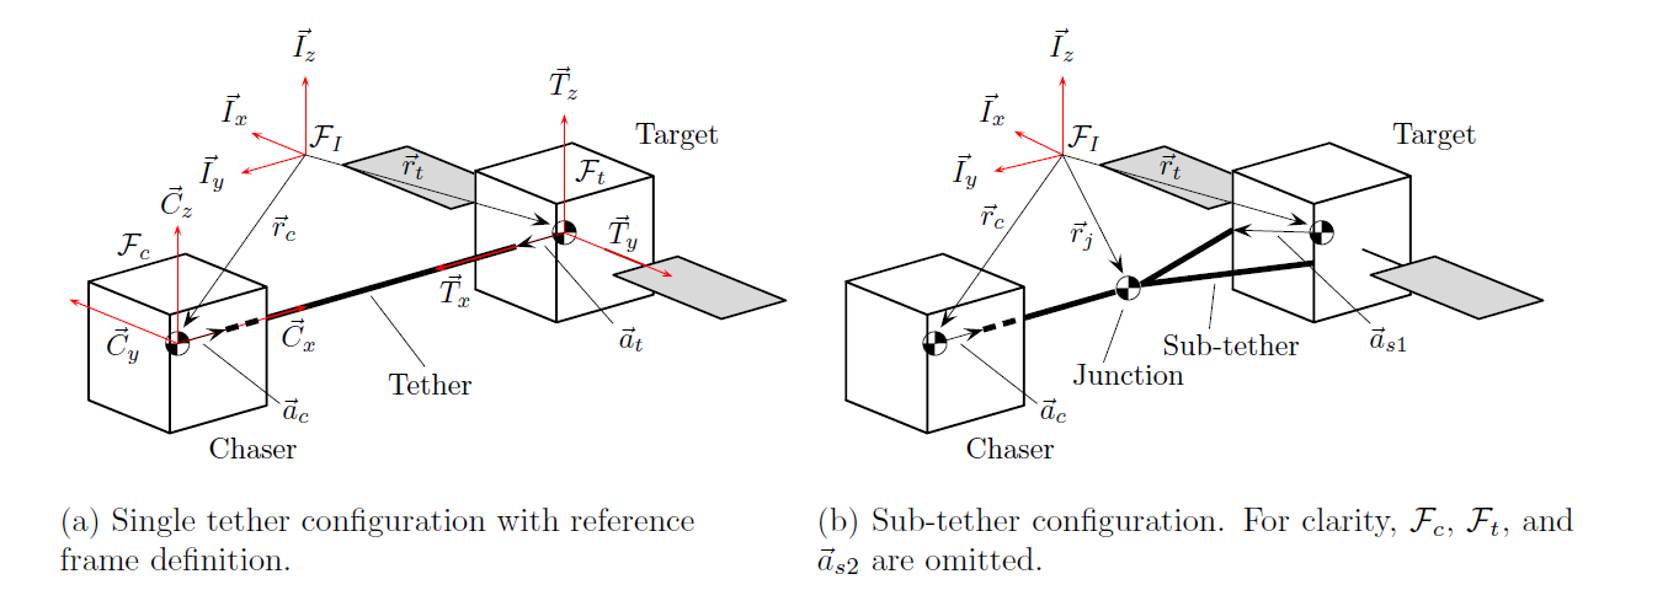
\includegraphics[width=\textwidth]{fig/simulation/ReferenceFrame}
\caption{Reference frame and vector definition for planar dynamics modeling}

\end{figure}
When we let our chaser vehicle connect with target vehicle using tether, the consumption of angular momentum becomes faster and the deorbiting gets quicker.  
So we can say that chaser vehicle plays as a role of active debris remover.

Using different kind of tether configuration, the effect of deorbiting target vehicle can be quite different.In Hovell's article, single tether confguration and sub-tether configuration are compared. The sub-tether configuration is like harpoon. The main tether links the Chaser vehicle with the junction point, which will be modeled as a point mass later.Two seperate tethers link the junction and Target vehicle. The proposed sub-tether configuration can enhance the deorbiting mechanism, reducing the target tether angle and angular rate of target and finally dissipating angular momentum from the system much more quickly.  
\section{Physical Model Assumption}

\begin{enumerate}
\label{simu-assumption}
\item Massless tether, Constant end-body mass and visco-elastic tether\\

The tether is assumed as massless since it is much more lighter than end-body satellites.  The single tether and sub-tether are modeled as nonlinear spring. The spring force are related to tether stretch and the relationship is set as visco-elastic.

\item Three degree of freedom for Chaser vehicle and Target vehicle\\

Only three degree of freedom is considered in this case which means the satellite can only do translational motion along X axis and Y axis and rotational motion about the Z axis. This assumption makes the dynamics modeling of satellite much easier. The two satellites, target and chaser, are at the same level height which means there is no translational motion along Z axis i.e the z = 0. Similarly, the rotational motion about X axis and the rotational motion about Y axis are not con
\item No external forces applied to the center of mass of the whole tethered satellite system\\

In the tether satellite system, the force of tether and the chaser's control force are force source. No external force, such as gravational force and distrubance force applied to the center of mass of the whole system. 
\item The Inertia matrix is constant

\item Body frame of each of the end-masses is aligned with the principal axes of the end-masses
\end{enumerate}

\begin{figure}[ht]
\centering
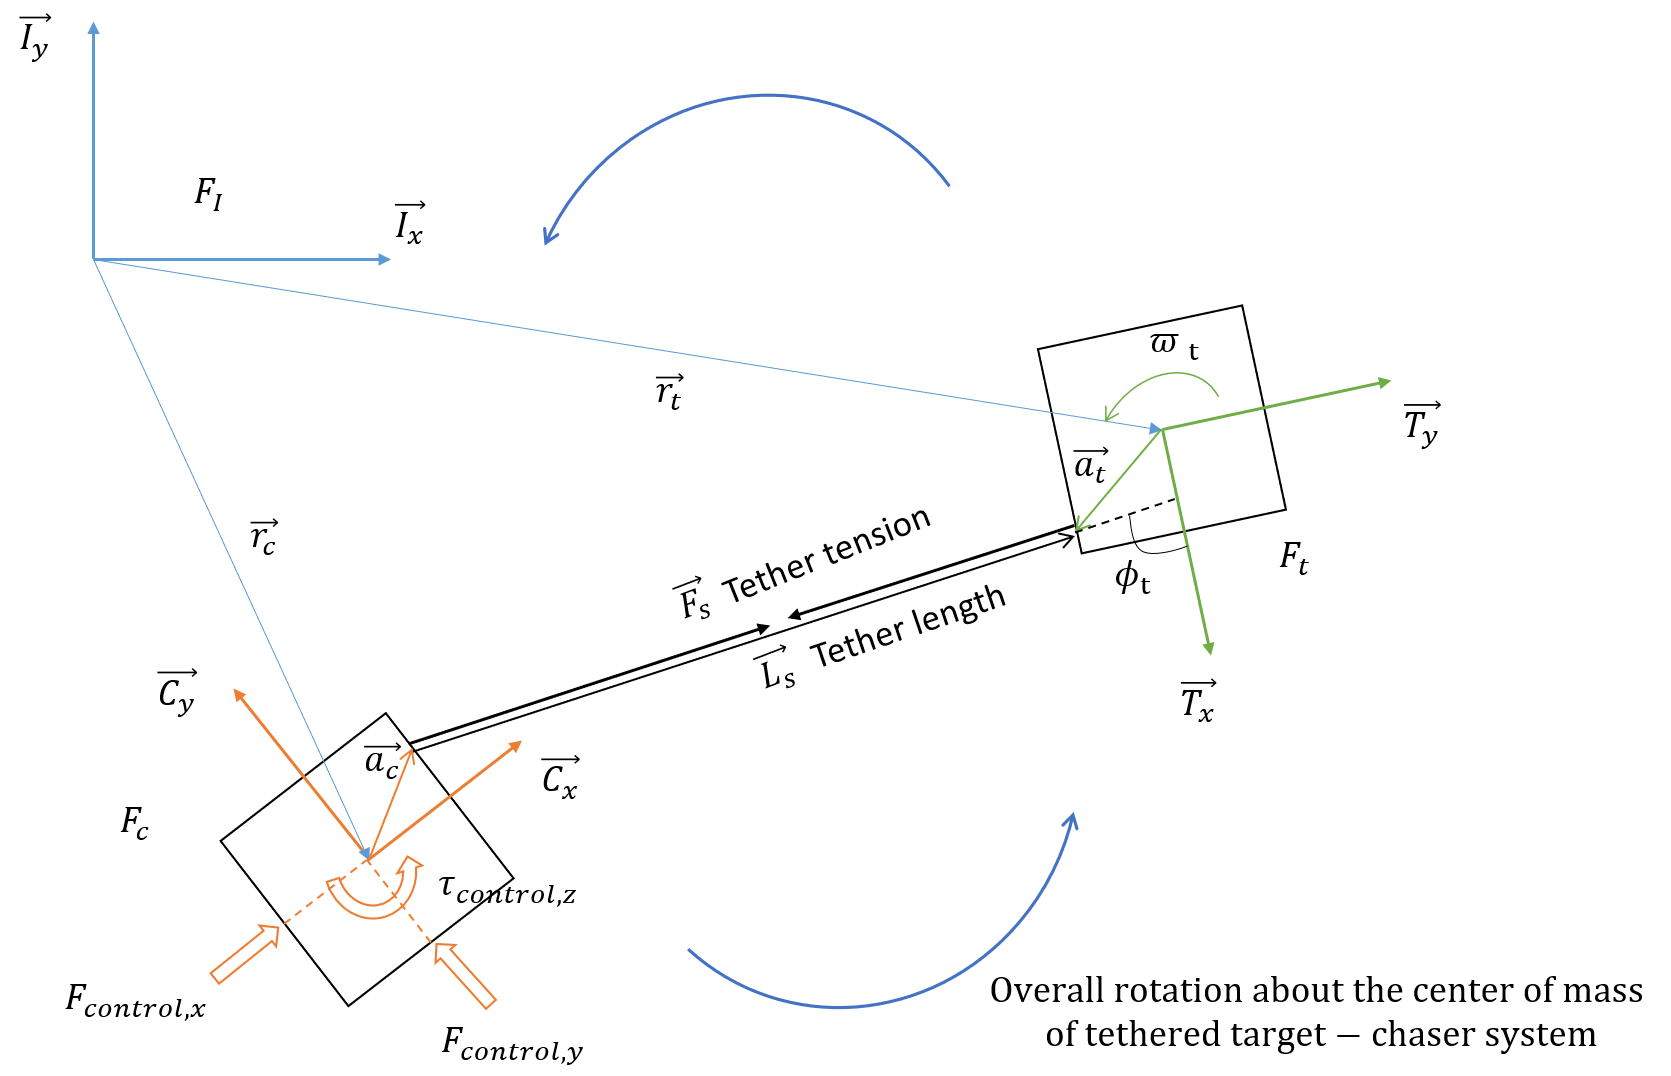
\includegraphics[width=0.8\textwidth,right]{fig/simulation/illustration.png}
\caption{Definition of the Inertial frame, Chaser body frame and Target body coordinate systems}
\label{simu-illustration}
\end{figure}


There are three coordinate systems defined in the article and all of them are defined as right-handed system. Between two different coordinate systems the attitude matrix $A(\theta)$ is the transformation matrix whcih used to rotate the vector components from a body frame to Inertial frame. 
\begin{equation}
A(\theta) =
	\begin{bmatrix}
	\cos(\theta) & -\sin(\theta) \\
	\sin(\theta) & \cos(\theta)
	\end{bmatrix}
\end{equation}

	The point where tether attached the Chaser vehicle or Target vehicle is called attached point. This point is fixed in the body frame so that we can use tether attachment vector with respect to the body centor of mass to describe this attach point. The tether attachment vector is denoted as $a$.
The attitude $\theta$  of a body frame ($F_C$ for the chaser or $F_T$ for of the target) is the angle of rotation between the body frame relative to the Inertial frame $F_I$ about the z-axis where the z-axis of all inertial and body frames are parallel. The transformation of vectors from body frame to Inertial frame is using the equation  $\mathbf{x_I}=A(\theta)\mathbf{x_b}$ which $I$ means Inertial frame and $b$ means body frame.
\boldmath
\begin{enumerate}

\item Reference inertial frame $F_I$ Coordinates\\		
\begin{center} $\textbf{I} =[I_x, I_y, I_z]$ \end{center}
\textbf {$F_I$} is fixed. The position of origin point and direction of three axes will not change with time.    


\item Reference inertial frame $F_T$ Coordinates\\		
\begin{center} $\textbf{T} =[T_x, T_y, T_z]$ \end{center}
\textbf{$F_T$} denotes the Target body-fixed frame. The origin point of \textbf{T} is at the center of mass of the Target vehicle. The x axis of $F_T$ is pointed to the chaser at the beginning. 

\item Reference inertial frame $F_C$ Coordinates\\		
\begin{center} $\textbf{C} =[C_x, C_y, C_z]$ \end{center}
\textbf{$F_C$} denotes the Chaser body-fixed frame.The origin point of \textbf{C} is at the center of mass of the Target. The x axis of $F_C$ is pointed to the target at the beginning. 
\end{enumerate}
\unboldmath

\section{Motion governing equation and Physics model for the system}

This section talks about the details of physical model and the motion governing equation

\subsection{Motion governing equation}

The governing equations are Newton's second law and Euler's equation.

Using the Newton's second law we can get that the sum of force vector components acting on any body in Inertia Frame,$\mathbf{F}$, equals the mass of the satellite $m$ times the resulting acceleration vector components in Inertia Frame $\ddot{r}$ i.e. $ \mathbf{F} = m\mathbf{\ddot{r}}$

Similarly, using the Euler's equation we can get that the torque of the chaser's body or target's body as a result of the force exerted by the tether and/or the chaser's control actuator equals z axis Principal moment of inertia multiplied by Angular velocity of an end-mass/satellite relative to the inertial frame (which also equals to the angular velocity relative the body frame) i.e. $J_{zz} \dot{\omega} = \tau_z$ 

\subsection{Physics model for the system}

The whole system is modeled as a nonlinear stiffness spring-damper system. The damping coefficient of the damper is constant. The tether is made of 56\% polyester and 44\% rubber. The spring constant $k$ has strong nonlinearity. 

\begin{itemize}

\item The spring constant changes as the extension of tether change 

\item When tether is extended, the spring force $F_{spring} = k\times $(length of stretched tether - tether natural length)

\item $F_{spring} = 0$ when tether is slacked

\end{itemize}

\begin{figure}[htbp]
\centering
\begin{minipage}[t]{0.48\textwidth}
\centering
\includegraphics[width=6cm]{fig/simulation/Systemmodel}
\caption{System model}
\label{simu-systemmodel}
\end{minipage}
\begin{minipage}[t]{0.48\textwidth}
\centering
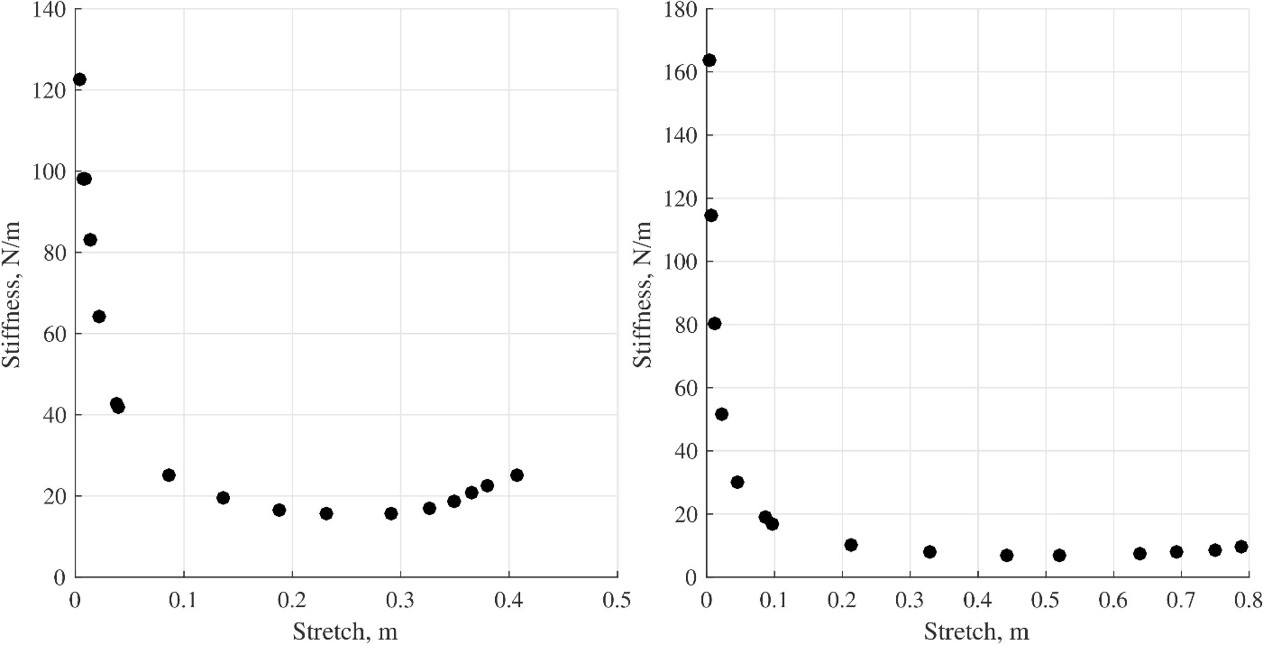
\includegraphics[width=6cm]{fig/simulation/StiffnessStetchRelation}
\caption{Stiffness stetch relation}
\end{minipage}
\end{figure}

\subsection{Force and Torque analysis}

1. For the Target vehicle, it only received the force of tether tension which denoted as $\mathbf{-\overrightarrow{F_S}}$. The torque $\tau_t$ is the torque made by tether tension about the center of mass of the target body.
\begin{equation}
\tau_t = a_{t,y}F_{s,x}^t - a_{t,x}F_{s,y}^t
\end{equation}
\quad $F_{s}^t$ is the tether force expressed in $F_t$ i.e. $F_{s}^t = A(\theta_t)^TF_S$\\
\quad\quad $F_{s,x}^t,F_{s,y}^t$ are the x and y components of $F_{s}^t$ in $F_T$, respectively.   

2. For the Chaser vehicle tether force $\mathbf{\overrightarrow{F_S}}$ and active control force $\mathbf{\overrightarrow{F_{control}}}$both exist. The torque also consists of two parts $\tau_{control}$ and  $\tau_{c}$. The $\tau_{control}$ and $\mathbf{\overrightarrow{F_{control}}}$ are the active control way that research can design in order to get the better deorbiting performance.
\begin{equation}
\tau_c = a_{c,x}F_{s,x}^c - a_{c,y}F_{s,x}^c
\end{equation}

\quad $F_{s}^c$ is the tether force expressed in $F_c$ i.e. $F_{s}^c = A(\theta_c)^TF_S$\\
\quad $F_{s,x}^c,F_{s,y}^c$ are the x and y components of $F_{s}^c$ in $F_c$, respectively.

\begin{figure}
\centering
\includegraphics[width=\textwidth]{fig/simulation/flowchart}
\caption{Flowchart of the calculation process}
\label{simu-flowchart}
\end{figure}

\subsection{Tether length, tether tension and tether torque}

According to Figure\ref{simu-illustration}, changing all the vectors in the Inertial frame then the vector form of tether length can be written as follows:

\begin{equation} \overrightarrow{L_S} = -(\overrightarrow{r_c} + A(\theta_c)\overrightarrow{a_c})+(\overrightarrow{r_t} + A(\theta_t)\overrightarrow{a_t})\end{equation}
 

As Figure \ref{simu-systemmodel} described before, the damping mechanism of tether results in the damping force: $c(\Delta\overrightarrow{v}\cdot \frac{\overrightarrow{L_S}}{\norm{\overrightarrow{L_S}}}) $. It results from damping factor times the velocity change in the tether's direction

The tether tension is: 
\begin{equation} \overrightarrow{F_S} = \bigl(k(\norm{\overrightarrow{L_S}} - L_{s,nature}) + c(\Delta\overrightarrow{v} \cdot 
	\frac{\overrightarrow{L_S}}{\norm{\overrightarrow{L_S}}})
	\bigr)
	\frac{\overrightarrow{L_S}}{
	\norm{
	\overrightarrow{L_S}
	}
	}
\end{equation}
$\frac{\overrightarrow{L_S}}{\norm{\overrightarrow{L_S}}}$ is the unit vector of the tether.$\Delta\overrightarrow{v}$ is the difference of the time derivative of two body's absolute postion. 
\begin{equation}\Delta\overrightarrow{v} = \frac{d}{dt}(\overrightarrow{r_t}+A(\theta_t)\overrightarrow{a_t}) - \frac{d}{dt}(\overrightarrow{r_c} + A(\theta_c)\overrightarrow{a_c}) = \overrightarrow{v_t} + \frac{d}{dt}(A(\theta_t))\overrightarrow{a_t}-\overrightarrow{v_c}-\frac{d}{dt}(A(\theta_c))\overrightarrow{a_c}\end{equation}
Since the derivate is used for the angle, we can rewrite the $\frac{d}{dt}(A(\theta_t))\overrightarrow{a_t}$ in terms of angular rate and tether attachment vector.
\begin{equation}\frac{d}{dt}(A(\theta_t))\overrightarrow{a_t} = \frac{d}{dt}
\left(
\begin{bmatrix}
\cos(\theta_t) & -\sin(\theta_t)\\
\sin(\theta_t) & \cos(\theta_t)
\end{bmatrix} \right)
\overrightarrow{a_t} =
\begin{bmatrix}
\cos(\theta_t) & -\sin(\theta_t)\\
\sin(\theta_t) & \cos(\theta_t)
\end{bmatrix}
\left(
\begin{array}{c}
-\omega_ta_{t,y}\\
\omega_ta_{t,x}
\end{array}\right)
\end{equation}
which means that 

$$\frac{d}{dt}(A(\theta_t))\overrightarrow{a_t} = A(\theta_t)\left(
\begin{array}{c}
-\omega_ta_{t,y}\\
\omega_ta_{t,x}
\end{array}\right) \frac{d}{dt}(A(\theta_c))\overrightarrow{a_c} = A(\theta_c)\left(
\begin{array}{c}
-\omega_ca_{c,y}\\
\omega_ca_{c,x}
\end{array}\right)$$

Tether torque can be written as the time derivative of system angular momentum. It equals the time derivative of system angular momentum with regard to the relative moving coordinate system plus the moving frame's absolute angular velocity times the angular momentum. In this case the moving frame just has translational motion in Inertia frame. The moving frame's absolute angular velocity doesn't exist in this case. 
\begin{equation} M = \frac{dH}{dt} = \dot{H_{relative}} + \Omega \times H\\
		=\dot{H_{relative}} =\frac{J_{zz}\omega}{dt}= J_{zz}\dot{\omega}
\end{equation}
The torque in Inertial frame equals the torque in body frame.
For the rigid body i In the inertial frame, the euler's equation gives us the relationship between the exerted torque $\tau$ and resulted angular acceleration $\dot{\omega}$ .i.e. $J_i\dot{\omega} + \omega_i \times J_i\omega_i=\sum\tau$

According to the assumption \ref{simu-assumption} we can simplified the Euler's equation as: $J_{izz}\dot{w_{iz}}=\tau_{iz}$	i can be c for chaser or t for target.
$\tau=a_i\times F^i_S$	$\tau_t = a_{t,y}F_{s,x}^t - a_{t,x}F_{s,y}^t$	$\tau_c = a_{c,x}F_{s,x}^c - a_{c,y}F_{s,x}^c$

\section{Control goal of Chaser vehicle}
To archieve the goal of deorbiting target satellite, the Chaser vehicle need to regulate and reduce the angle between tether and target so as to make the tether aligned with the target or force Chaser and target has the parellel surface. To reduce the angular rate of target vehicle, dissipate angular momentume from the system and at last make the target go to lower altitude orbit.
\begin{figure}
\centering
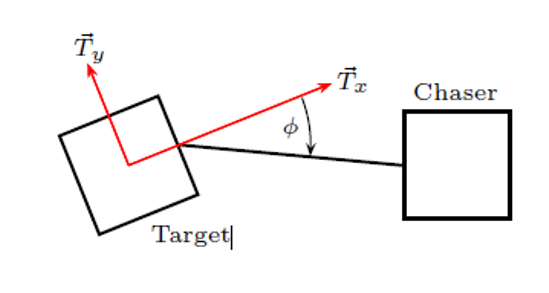
\includegraphics{fig/simulation/TetherTargetAngle}
\caption{Positive tether target angle}
\end{figure}
The easiest way is to use the proportional-derivative controller for the position and altitude contro of the tether.
The force controller uses the difference between desired chaser radius vector and actual chaser radius vector as the feedback signal. The force $\overrightarrow{F_{s,control}}$ equals $\mathbf{K_P}\left[\overrightarrow{r_{des}(t)}-\overrightarrow{r_c(t)}\right]+\mathbf{K_D}\left[\overrightarrow{\dot{r_{des}(t)}}-\overrightarrow{\dot{r_c(t)}}\right]$
Similarly the torque controller uses the desired chaser attitude angle and actual chaser attitude angle as the control feedback signal.

$$\tau_{control} =K_{P,\theta}\left[\theta_{des}(t)-\theta_c(t)\right] + K_{D,\theta}\left[\dot{\theta_{des}(t)}-\dot{\theta_c(t)}\right]$$

$K_P,K_{P,\theta},, K_D,K_{D,\theta}$ are the Proportional gain matrix and the Derivative gain matrix respectively. These matrix value are designed and tuned by designer for the special case.

\section{MATLAB Implementation}
In this section, the MATLAB simulation case is implemented. To simplified the study, the implementation case use only one controller. The thrust stabilization only use force controller. The Tether Satellite System Spin Stabilization only use torque control, commanding the chaser to continually point its $C_x$  axis toward the target. In the real case the controller can be the combination of these two kinds. Here we just implemented the Thrust stabilization of single tether for illustration the problem.

The detail MATLAB code is in the Appendix. Symbols have the same meaning and constant values are not changed, as\cite{hovell2017experimental}. 

\section{Thrust stabilization}

The chaser is designed as uniformly accelerated motion for simplicity. The motion can be replayced by any other arbitarily defined motion. $$\overrightarrow{r_{des}(t)}=\overrightarrow{r_0}+\overrightarrow{d}\frac{t^2}{2}$$ d is the acceleration got from the desired final radius vector, the initial radius vector and assigned time for motion, $\overrightarrow{d} = \frac{2(\overrightarrow{r_{final}}-\overrightarrow{r_0})}{t^2}$.
$\overrightarrow{\dot{r_{des}}(t)}=\overrightarrow{d}t$ 


\begin{figure}[htbp]
\centering
\begin{minipage}[t]{0.48\textwidth}
\centering
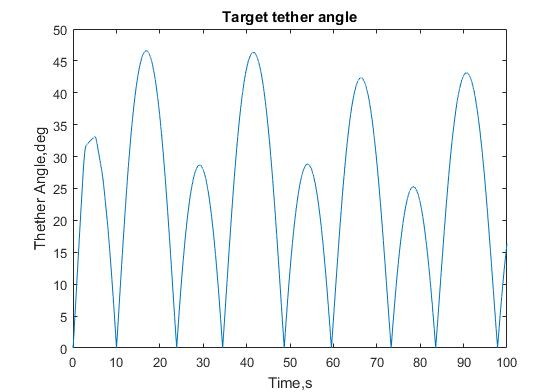
\includegraphics[width=6cm,height=6cm]{fig/simulation/ThrustStable/Targettetherangle.jpg}
\end{minipage}
\begin{minipage}[t]{0.48\textwidth}
\centering
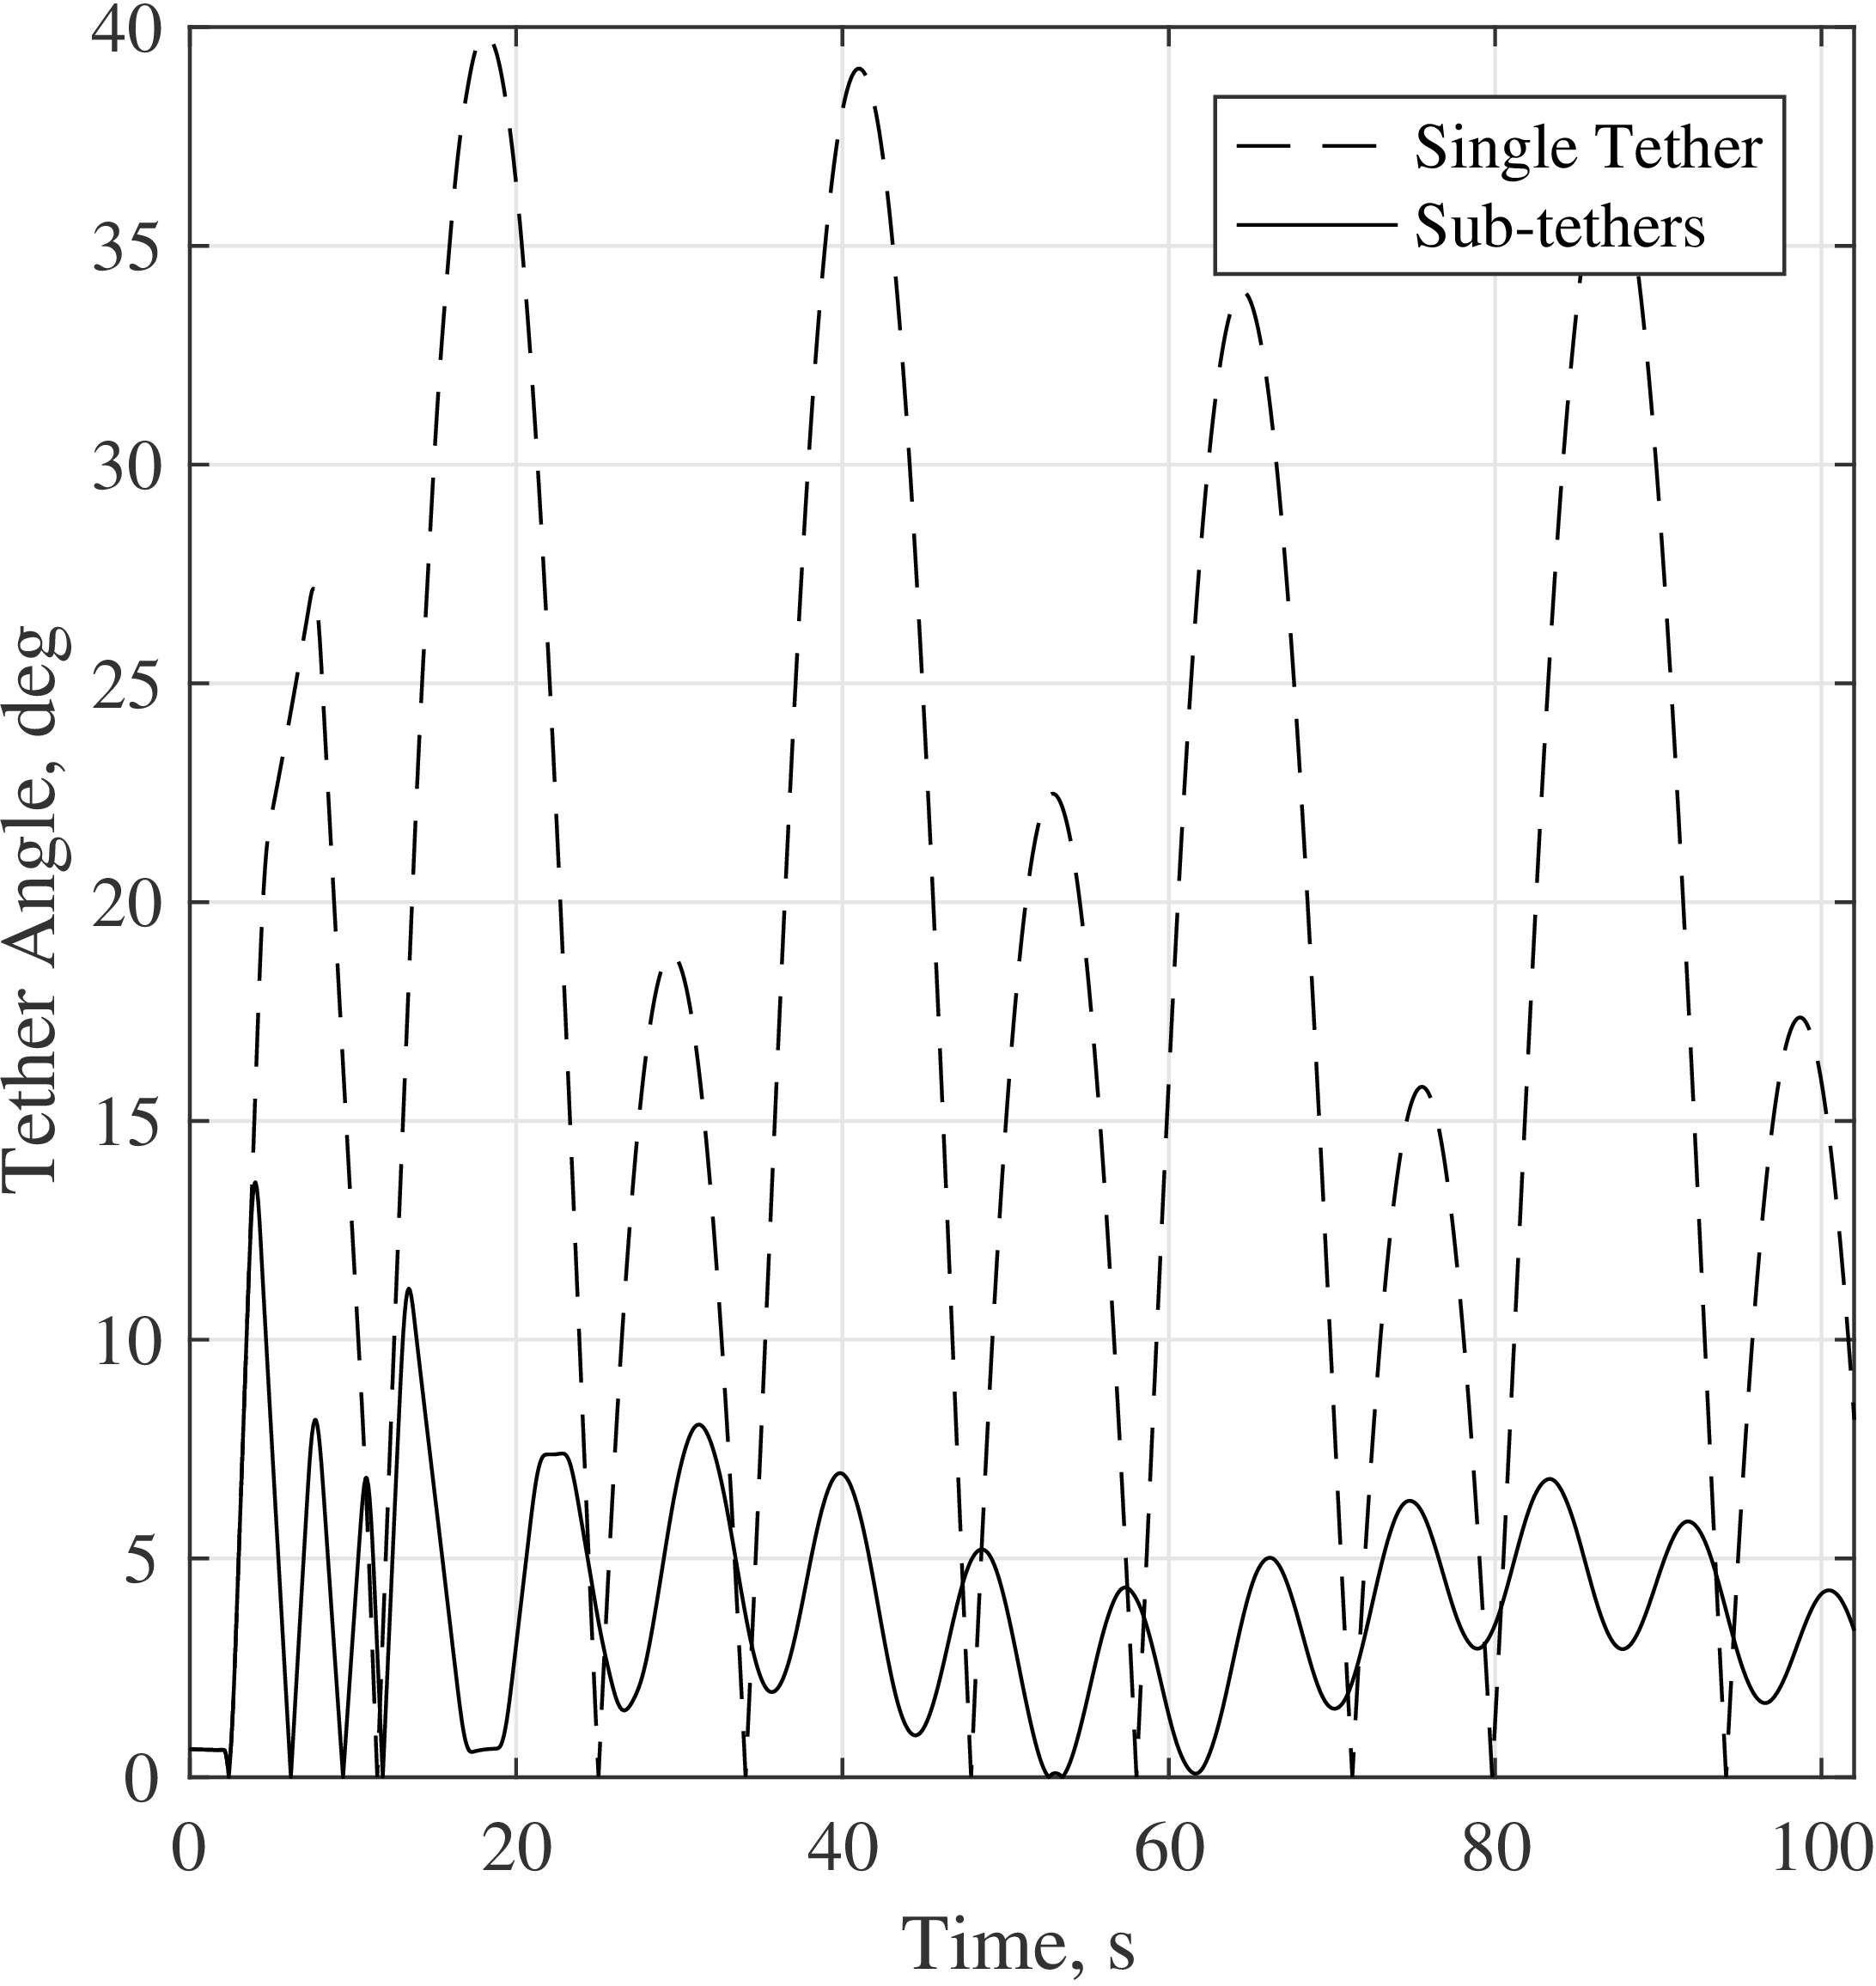
\includegraphics[width=6cm,height=6cm]{fig/simulation/ThrustStable/Targettetheranglesample.jpg}
\end{minipage}
\caption{Comparison of Target tether angle. Left: Kaiwen	Right: Hovell}
\end{figure}

\begin{figure}[htbp]
\centering
\begin{minipage}[t]{0.48\textwidth}
\centering
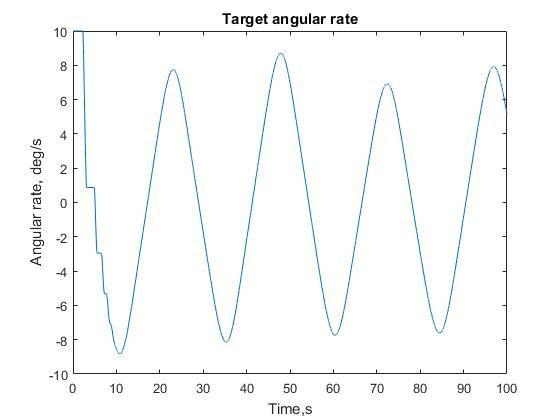
\includegraphics[width=6cm,height=6cm]{fig/simulation/ThrustStable/Targetangularrate.jpg}
\end{minipage}
\begin{minipage}[t]{0.48\textwidth}
\centering
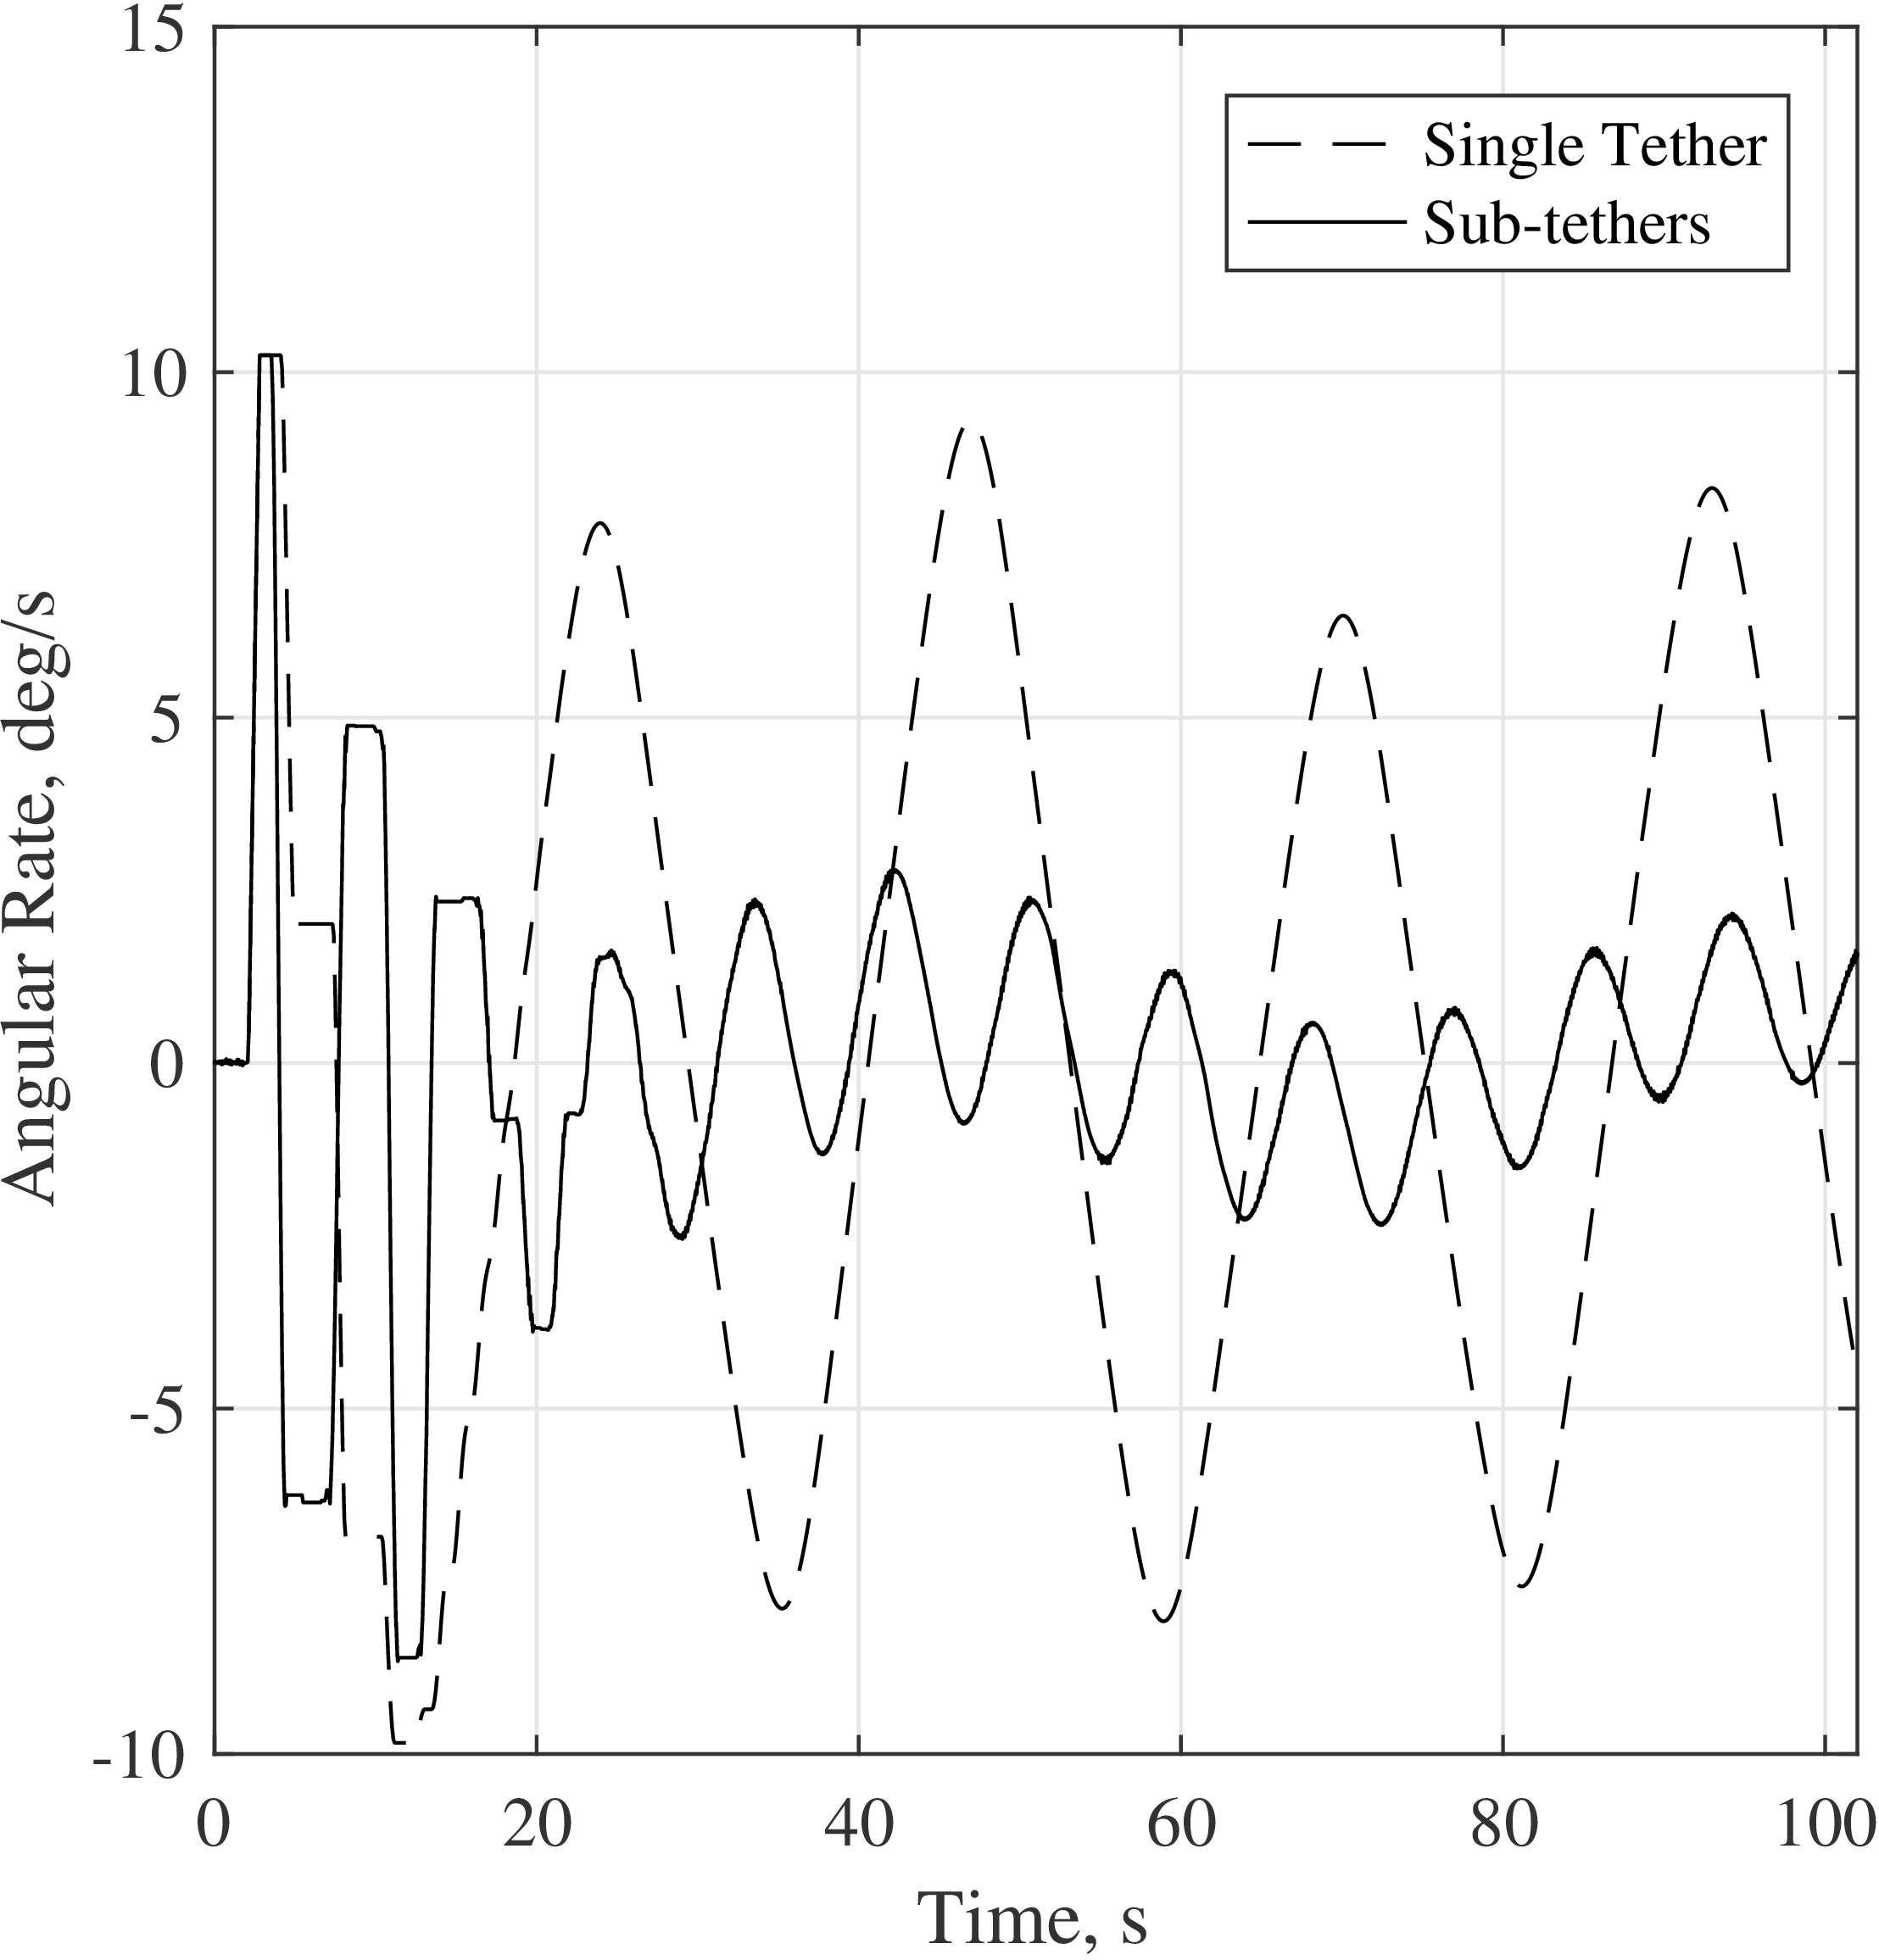
\includegraphics[width=6cm,height=6cm]{fig/simulation/ThrustStable/Targetangularratesample.jpg}
\end{minipage}
\caption{Comparison of Target angular rate.		Left: Kaiwen	Right: Hovell}
\end{figure}

\begin{figure}[htbp]
\centering
\begin{minipage}[t]{0.48\textwidth}
\centering
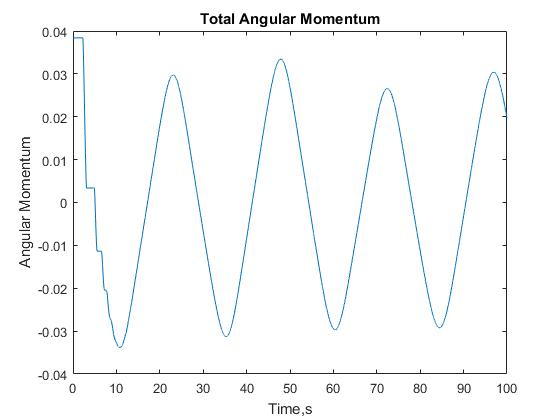
\includegraphics[width=6cm,height=6cm]{fig/simulation/ThrustStable/Totalangularmomentum.jpg}
\end{minipage}
\begin{minipage}[t]{0.48\textwidth}
\centering
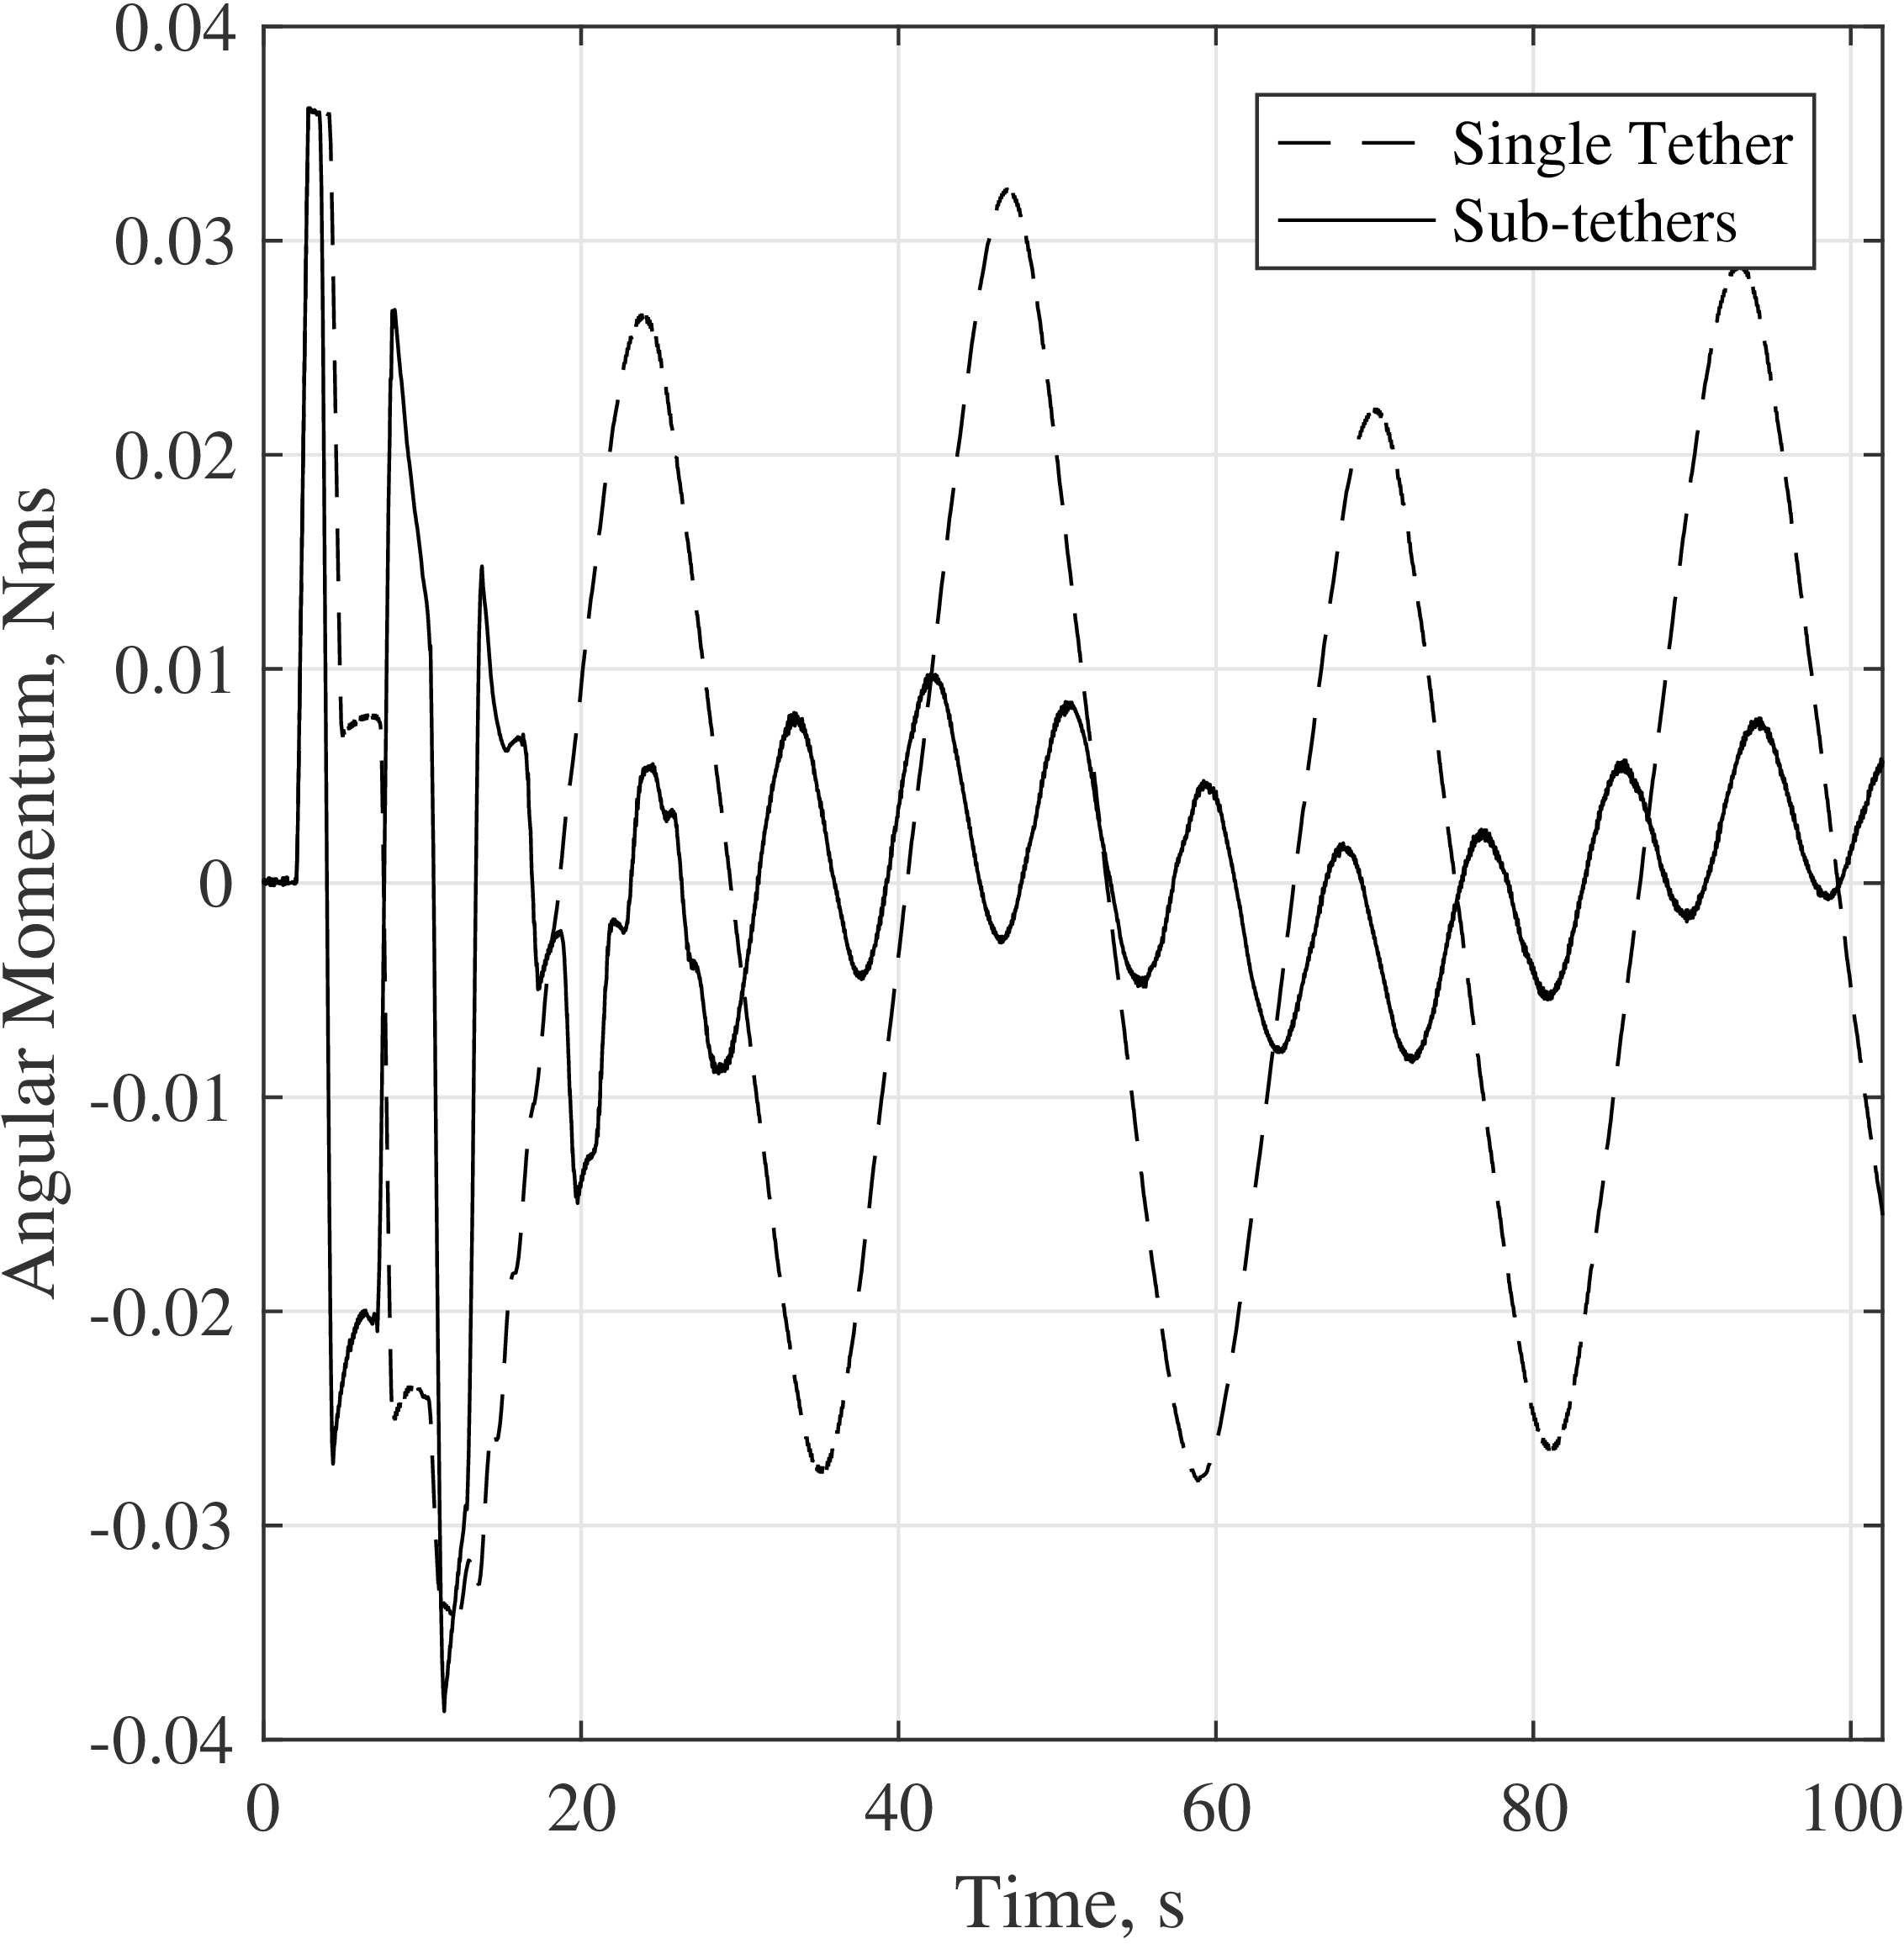
\includegraphics[width=6cm,height=6cm]{fig/simulation/ThrustStable/Totalangularmomentumsample.jpg}
\end{minipage}
\caption{Comparison of Total angular momentum.		Left: Kaiwen	Right: Hovell}
\end{figure}

\begin{figure}[htbp]
\centering
\begin{minipage}[t]{0.48\textwidth}
\centering
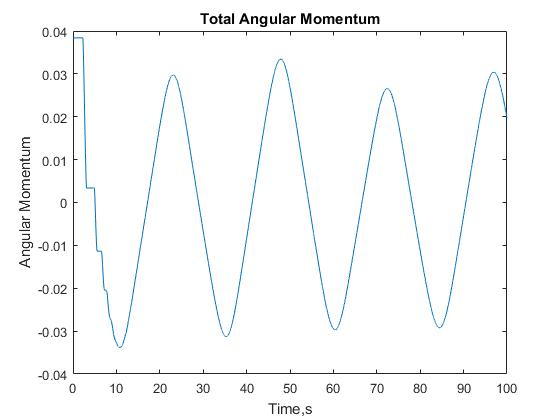
\includegraphics[width=6cm,height=6cm]{fig/simulation/ThrustStable/Totalangularmomentum.jpg}
\end{minipage}
\begin{minipage}[t]{0.48\textwidth}
\centering
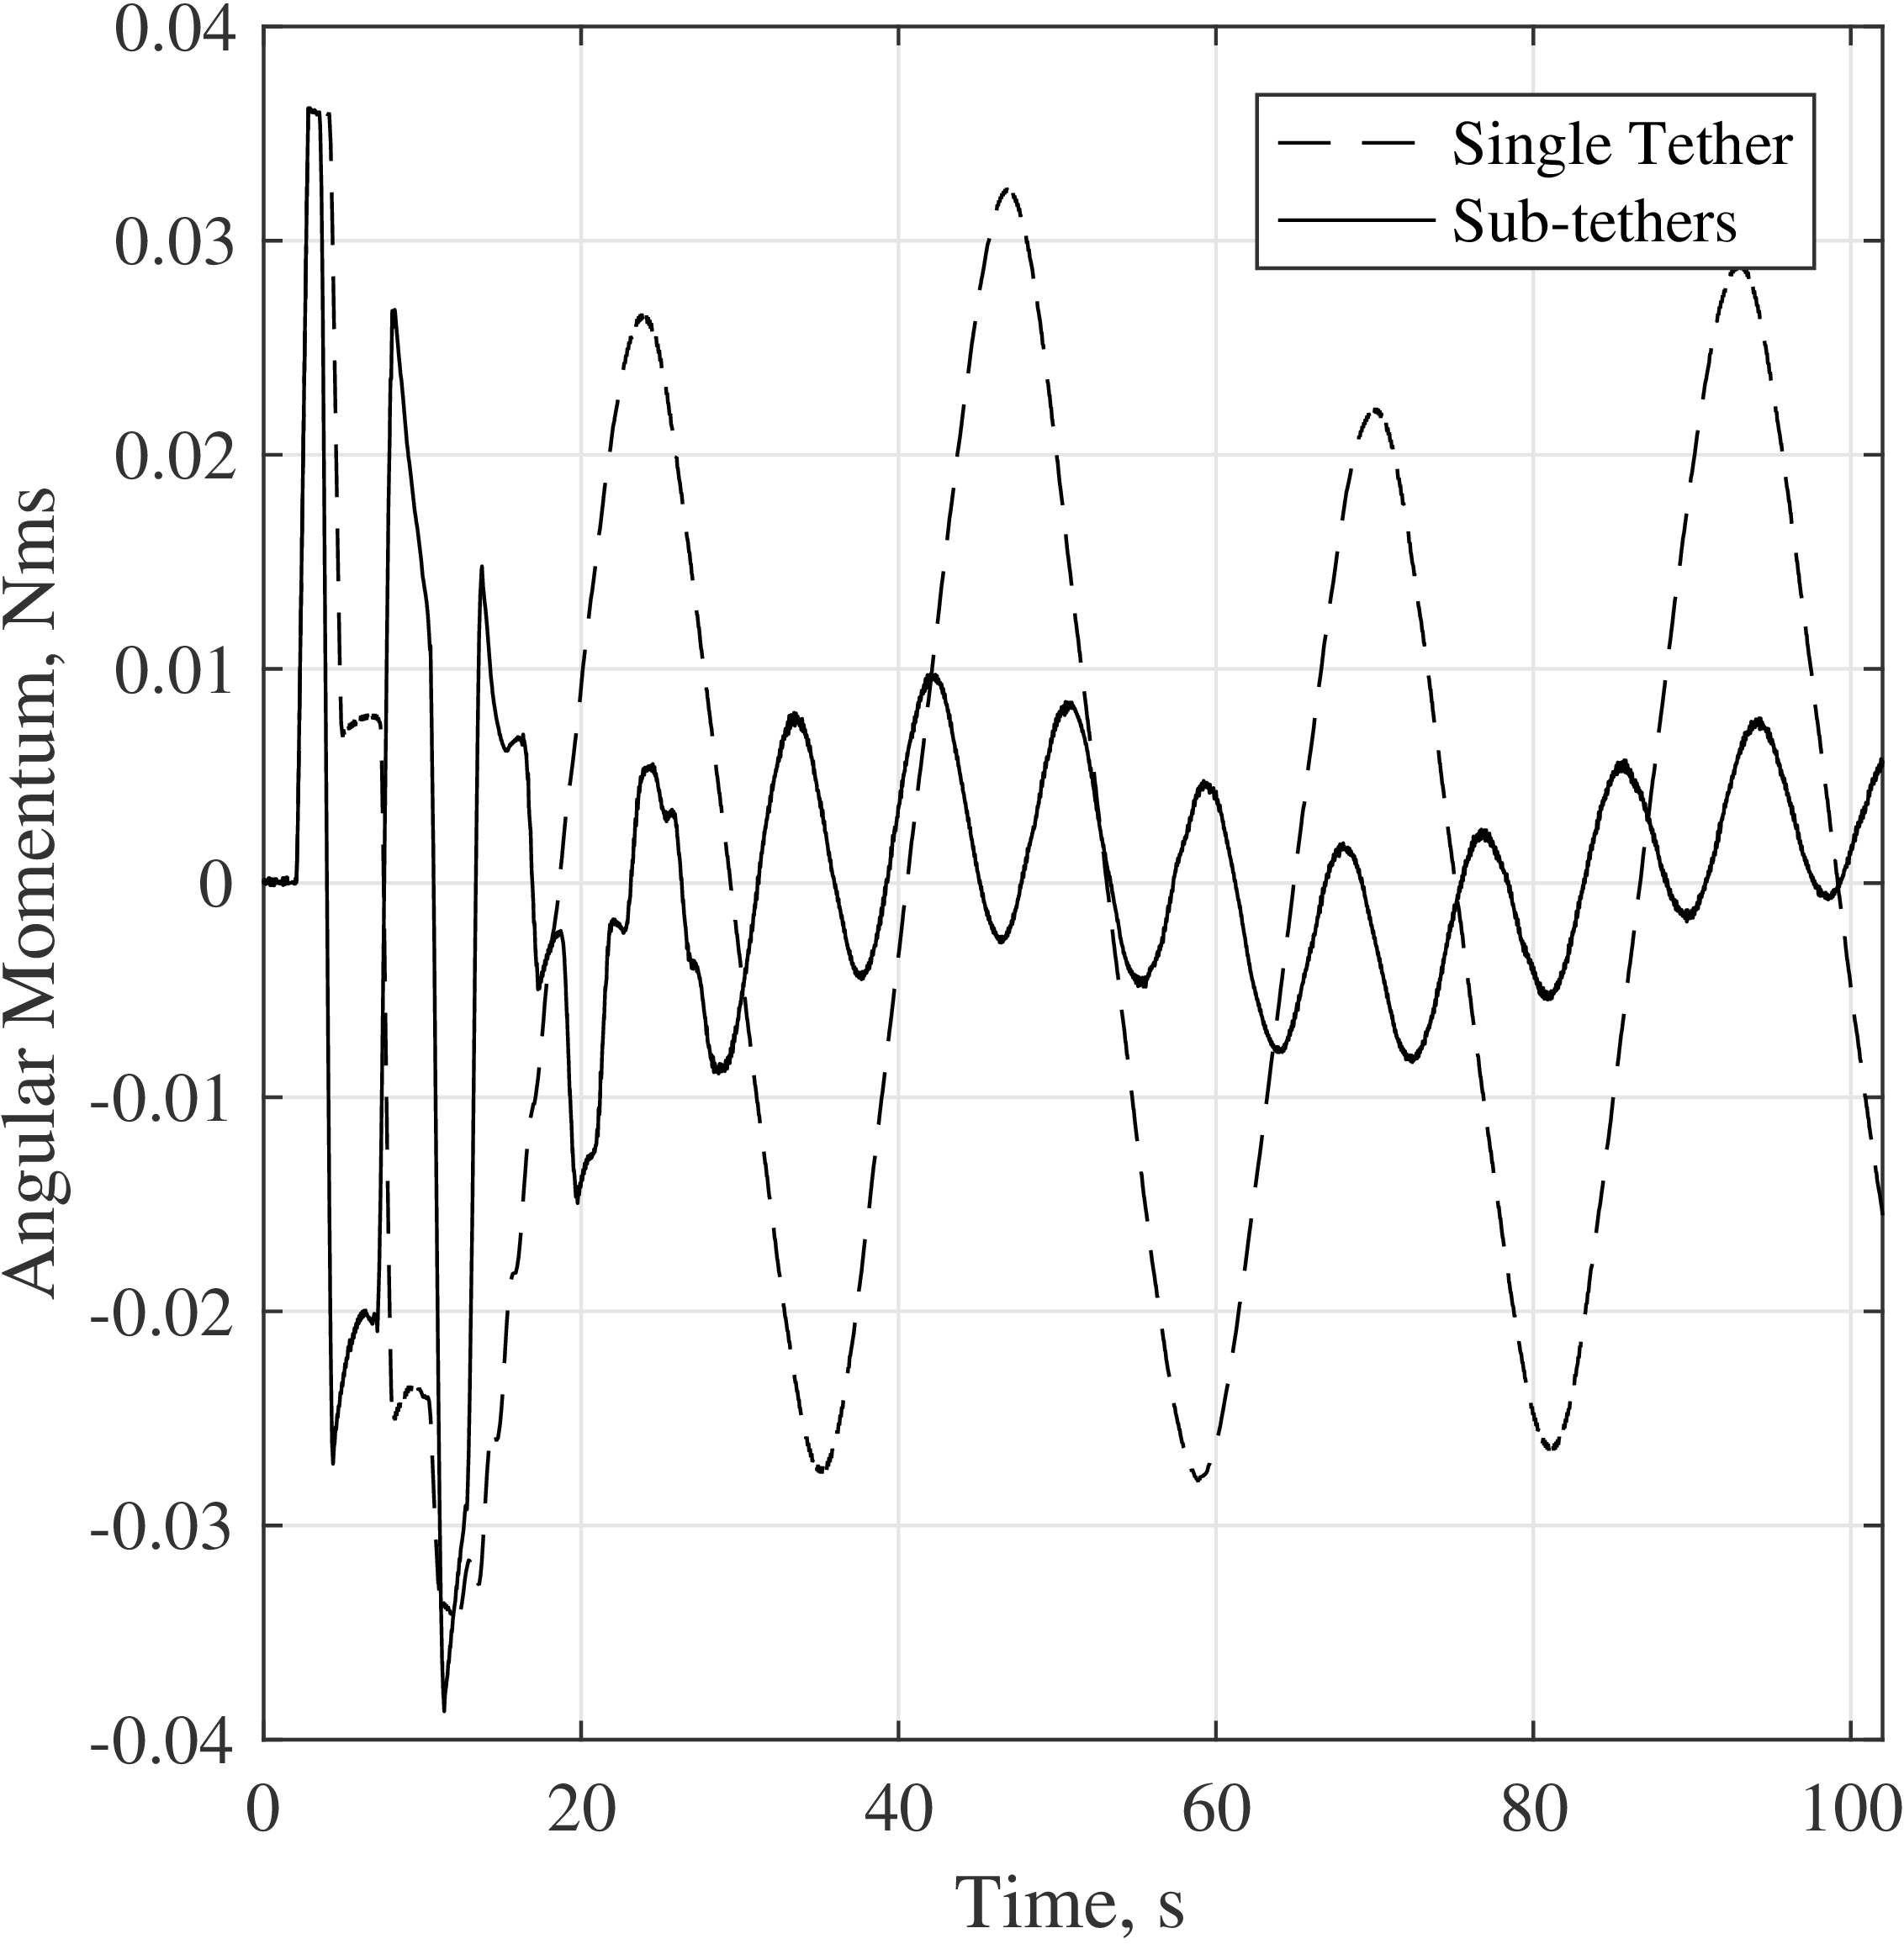
\includegraphics[width=6cm,height=6cm]{fig/simulation/ThrustStable/Totalangularmomentumsample.jpg}
\end{minipage}
\caption{Comparison of Total angular momentum.		Left: Kaiwen	Right: Hovell}
\end{figure}

\begin{figure}[htbp]
\centering
\begin{minipage}[t]{0.48\textwidth}
\centering
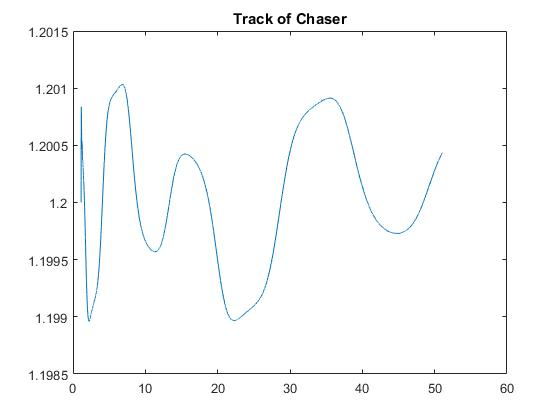
\includegraphics[width=6cm,height=6cm]{fig/simulation/ThrustStable/TrackofChaser.jpg}
\caption{Track of Chaser}
\end{minipage}
\begin{minipage}[t]{0.48\textwidth}
\centering
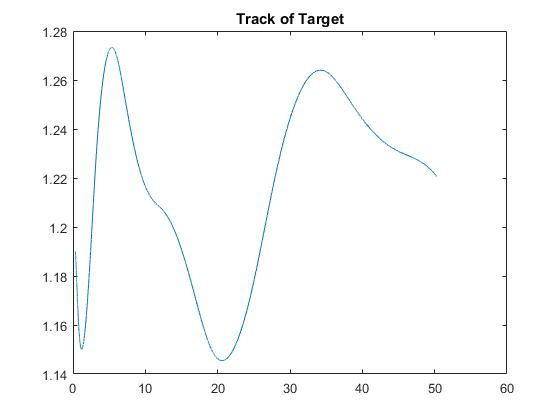
\includegraphics[width=6cm,height=6cm]{fig/simulation/ThrustStable/Trackoftarget.jpg}
\caption{Track of Target}
\end{minipage}
\end{figure}

From the figure comparison, we know that the effect of implementation is quite well.


\newpage

\chapter{Design of Experiment}\label{sec-DOE}
\chapter{Appendix}\label{section-appendix} 
\section{MATLAB}
\begin{lstlisting}
% This code is an implementation of Thrust Stabilization
% for single tether
% Hovell, K, and Ulrich, S. (2017)
% "Experimental Validation for Tethered Capture of the Spinning Space Debris"
% AIAA SciTech Forum, AIAA Guidance, Navigation, and Control Conference, Grapevine, Texas. 9 ?13 January
% Paper no AIAA 2017-1049.

% ======
% Nomenclature:
% Jzzt = Moment of inertia, target about z-axis 
% Jzzc = Moment of inertia, chaser about z-axis

% mt = Mass of the target
% mc = Mass of the chaser
% mj = Mass of the junction

% thetac0 = Initial angle of the chaser 
% thetat0 = Initial angle of the target

% TS = Time step

% Lm0= unstretched length of the main tether
% Ls10 = unstretched length of the sub tether 1
% Ls20 = unstretched length of the sub tether 2
% Ls0 = unstretched length of the single tether

% ac = tether attachment point to body chaser with respect to chaser's
% center of mass
% as1 = tether attachment point to body sub tether 1 with respect to
% sub-tether1's center of mass
% as2 = tether attachment point to body sub tether 2 with respect to
% sub-tether2's center of mass
% at = tether attachment point to body target with respect to
% target's center of mass

% csingle = damping coefficient for single tether
% csub = damping coefficient for sub tether

% KPtheta = proportional gain matrix for the theta 
% KDtheta = derivative gain matrix for the theta
% KP = proportional gain matrix for the position
% KD = derivative gain matrix for the postion

% ======
% Define initial conditions and TSS parameters for all simulations and
% experiment:

%in Kg·m^2
Jzzt=0.22; 
Jzzc=0.30; 

%in Kilogram
mt=12.19; 
mc=17.24; 
mj=0.01;

%in Degree
thetac0=180; 
thetat0=0;

% in Second
TS=0.004; 

%in Meter
Lm0=0.28; 
Ls10=0.28; 
Ls20=0.28;  
Ls0=0.54; 
ac=[0.135;-0.009];
as1=[0.110;0.127];
as2=[0.113;-0.094];
at=[0.110;0.016];

% in Newton·second/meter
csingle=3.0; 
csub=0.9;

KPtheta=0.33;
KDtheta=0.56;
KP=[19.1 0;0 19.1];
KD=[32.7 0;0 32.7];

% ======
% Define initial conditions for Thurst Stabilization simulations and experiment
rt0=[0.35;1.19];
rc0=[1.10;1.20];
vt0=[0;0];
vc0=[0;0];
wt0=10; %degree/second
rf=[3.10;1.20];

% ======
% Initialization
% Simulation at time t=2s
% Nothing change in the first two seconds
rt=rt0;
rc=rc0;
vt=vt0;
vc=vc0;
thetat=thetat0;
thetac=thetac0;
Ls=rt+A(thetat)*at-rc-A(thetac)*ac;

% fai is the target tether angle
fai=norm(atand(Ls(2)/Ls(1))-thetat);



wt=wt0;
wc=0;
t=0; % It started to simulate at T=2, which seem it as t=0;
Fs=[0;0];

% AngularMomentum 
% In radius

AngularMomentum = Jzzt * wt/57.3 + Jzzc * wc/57.3 ; 

accelerationc=[0;0];
accelerationt=[0;0];
angularaccelerationt=0;
taot=0;
Fcontrol=[0;0];



for i=1:25000 % i* TS = the time , i is the number of the current time step
%record the data
recordt(i)=t;
recordrc(i,1)=rc(1);
recordrc(i,2)=rc(2);
recordrt(i,1)=rt(1);
recordrt(i,2)=rt(2);
recordthetat(i)=thetat;

recordwt(i)=wt;
recordFs(i,1)=Fs(1);
recordFs(i,2)=Fs(2);

recordLs(i,1)=Ls(1);
recordLs(i,2)=Ls(2);


recordvc(i,1)=vc(1);
recordvc(i,2)=vc(2);

recordvt(i,1)=vt(1);
recordvt(i,2)=vt(2);

recordaccelerationc(i,1)=accelerationc(1);
recordaccelerationc(i,2)=accelerationc(2);
recordaccelerationt(i,1)=accelerationt(1);
recordaccelerationt(i,2)=accelerationt(2);

recordangularaccelerationt(i)=angularaccelerationt;

recordtaot(i)=taot;

recordFcontrol(i,1)=Fcontrol(1);
recordFcontrol(i,2)=Fcontrol(2);
recordfai(i)=fai;

recordAngularMomentum(i) = AngularMomentum ; 

%recordstiffness(i) = stiffness(norm(Ls)-Ls0);

%Ls is the vector which is from chaser to target, pointing at the target
Ls=rt+A(thetat)*at-rc-A(thetac)*ac;

% fai is target tether angle
fai=norm(-atand(Ls(2)/Ls(1))+thetat);


% Calculate the state of the tether 
% Hovell and Ulrich (2017) eqn 19
if (norm(Ls)-Ls0)>0 % tether is tensioned
    Fs=(stiffness(norm(Ls)-Ls0)*(norm(Ls)-Ls0)+...
        dot(csingle*(vt+A(thetat)*[-wt/57.3*at(2);wt/57.3*at(1)]-vc-A(thetac)*[-wc/57.3*ac(2);wc/57.3*ac(1)]),...
        Ls/norm(Ls))).*Ls/norm(Ls);
else % tether is slackness
    Fs=[0;0];
end

% Force on target due to tether tension:
% through center of mass
% referenced to the target's body frame
Fst=(A(thetat))'*Fs;
Fsc=(A(thetac))'*Fs;


% Torque on target due to tether tension:
% about the z-axis of body frame (which is parallel to the z-axis of inertial frame)
% through center of mass target
% referenced to target body frame (the torque referenced to the body is the same as to the inertial frame)
taot=at(2)*Fst(1)-at(1)*Fst(2); % Nm
taoc=ac(1)*Fsc(2)-ac(2)*Fsc(1); % Nm

% The control thrust of chaser vehicle
Fcontrol=KP*(rdes(t)-rc)+KD*(vdes(t)-vc);

% The control torque of chaser vehicle
taocontrol=KPtheta* (180 - thetac) + KDtheta*(0-wc)  ;
accelerationt=(-Fs/mt);
accelerationc=(Fs+Fcontrol)/mc;
angularaccelerationt=taot/Jzzt;
angularaccelerationc=(taoc+taocontrol)/Jzzc;

% position and angle update
rt=rt+vt*TS;
rc=rc+vc*TS;
thetat=thetat+wt*TS;
thetac=thetac+wc*TS;

vt=vt+accelerationt*TS;
wt=wt+angularaccelerationt*TS*(180/pi);%/degree t-1
vc=vc+accelerationc*TS;
wc=wc+angularaccelerationc*TS*(180/pi); %/degree t-1
AngularMomentum = Jzzt * wt/57.3 + Jzzc * wc/57.3;
t=t+TS;
end
recordt=recordt';
recordthetat=recordthetat';
recordwt=recordwt';


recordrc=recordrc';
recordrt=recordrt';
recordvc=recordvc';
recordvt=recordvt';
recordaccelerationc=recordaccelerationc';
recordaccelerationt=recordaccelerationt';
recordangularaccelerationt=recordangularaccelerationt';
recordangularaccelerationt=recordangularaccelerationt';
recordaccelerationc=recordaccelerationc';
recordaccelerationt=recordaccelerationt';
recordtaot=recordtaot';
recordFcontrol=recordFcontrol';

n=1;
figure(n)
plot(recordt,recordwt);
title('Target angular rate')
xlabel('Time,s')
ylabel('Angular rate, deg/s')
n=n+1;

figure(n)
plot(recordt,recordthetat)
title('angle of target')
n=n+1;

figure(n)
plot(recordt,recordrc(1,:))
title(' x position of the chaser')
n=n+1;

figure(n)
plot(recordt,recordrc(2,:))
title('y position of the chaser')
n=n+1;

figure(n)
plot(recordt,recordrt(1,:))
title('x position of the target')
n=n+1;

figure(n)
plot(recordt,recordrt(2,:))
title('y position of the target')
n=n+1;

figure(n)
plot(recordt,mod(recordfai,360))
title('Target tether angle')
xlabel('Time,s')
ylabel('Thether Angle,deg')
n=n+1;

figure(n)
plot(recordt,recordAngularMomentum)
title('Total Angular Momentum')
xlabel('Time,s')
ylabel('Angular Momentum')

n = n + 1;
figure(n)
plot(recordrc(1,:),recordrc(2,:))
title('Track of Chaser')

n = n+1;
figure(n)
plot(recordrt(1,:),recordrt(2,:))
title('Track of Target')

% The function gives the attitude matrix in terms of theta
% cos -sin; sin cos;

function attitude=A(sita)
attitude=[cosd(sita) -sind(sita);sind(sita) cosd(sita)];
end

% calculate the design radius vector of time t
% the goal is to reach the destination in 20s after t=2
function [rdes]=rdes(t)
rc0=[1.10;1.20];
rf=[3.10;1.20];
d=2.*(rf-rc0)./(20*20); %in 20s
[rdes]=(rc0+d.*(t*t/2));
end

% calculate the single tether stiffness(N/m) in terms of
% stretch(m)-independent variable 
% x=(||Ls||-Ls,0)
function stiff=stiffness(x)
originalstiffness=[163.500000000000,114.450000000000,80.2636363636363,51.3857142857143,29.9096000000000,18.8842500000000,17.0724030612245,10.1577253521127,8.06715957446808,7.09840970654628,6.99056826923077,7.22393661971831,8.06497910662824,8.78250400534045,9.58060266159696];
originalstretch=[0.00300000000000000,0.00600000000000001,0.0110000000000000,0.0210000000000000,0.0450000000000000,0.0860000000000001,0.0980000000000001,0.213000000000000,0.329000000000000,0.443000000000000,0.520000000000000,0.639000000000000,0.694000000000000,0.749000000000000,0.789000000000000];
stiff=spline(originalstretch,originalstiffness,x);
end

% calculate the design velocity of time t
% the goal is to reach the destination in 20s after t=2s
function vdes=vdes(t)
rc0=[1.10;1.20];
rf=[3.10;1.20];
d=2.*(rf-rc0)./(20*20); %in 20s
vdes=d*t;
end
\end{lstlisting}

\section{Arduino CSV Streaming Example}
\begin{lstlisting}
#include <ArdusatSDK.h>
#include <Wire.h>
#include <Arduino.h>


/*-----------------------------------------------------------------------------
 *  Setup Software Serial to allow for both RF communication and USB communication
 *    RX is digital pin 8 (connect to TX/DOUT of RF Device)
 *    TX is digital pin 9 (connect to RX/DIN of RF Device)
 *-----------------------------------------------------------------------------*/
ArdusatSerial serialConnection(SERIAL_MODE_HARDWARE_AND_SOFTWARE, 8, 9); 

/*-----------------------------------------------------------------------------
 *  Constant Definitions
 *-----------------------------------------------------------------------------*/
 
Acceleration accel;
Gyro gyro;
Magnetic mag;
Orientation orient(accel, mag);

void setup(void) {
  serialConnection.begin(57600);
  
  accel.begin();
  gyro.begin();
  mag.begin();
  orient.begin();
  serialConnection.println("Start of the loop");
  serialConnection.println("The acceleration x y z unit in m/s^2");
  serialConnection.println("The angular rate x y z unit in radian per second");
  serialConnection.println("The orientation roll pitch heading unit in degree");
}

void loop(void) {
  serialConnection.println(accel.readToCSV("Acceleration"));
  serialConnection.println(gyro.readToCSV("Gyro"));
  serialConnection.println(orient.readToCSV("Orientation"));
}

\end{lstlisting}
\section{MATLAB Serial REALTIME PLOTING} 
\begin{lstlisting} 
%% Pre-process
close all;  % close all figures
clear all;  % clear all workspace variables
clc;        % clear the command line
fclose('all'); % close all open files
delete(instrfindall); % reset com port 

%% Constatns
BAUDRATE = 57600; % Need to configure Xbee parts BD i.e. Interface Data Rate
INPUTBUFFER = 51200; %Unit in bytes. Definition:A location that holds all 
% incoming information before it continues to the CPU for processing; 
% Buffers used to store information before it processed


%% Initialize the stripchart
figure_acceleration = figure('Name','Acceleration');
axes_accelerationx = subplot(3,1,1); % Axes Object
xlabel(axes_accelerationx,'Time/ second')
ylabel(axes_accelerationx,'Accelerationx/ m/s^2')

axes_accelerationy = subplot(3,1,2);
xlabel(axes_accelerationy,'Time/ second')
ylabel(axes_accelerationy,'Accelerationy/ m/s^2')

axes_accelerationz = subplot(3,1,3);
xlabel(axes_accelerationz,'Time/ second')
ylabel(axes_accelerationz,'Accelerationz/ m/s^2')

h_ax = animatedline(axes_accelerationx,'MaximumNumPoints',Inf,'Marker','o','Color','red'); % animated line object
h_ay = animatedline(axes_accelerationy,'MaximumNumPoints',Inf,'Marker','+','Color','blue');
h_az = animatedline(axes_accelerationz,'MaximumNumPoints',Inf,'Marker','*','Color','green');

figure_gyro = figure('Name','Gyro');
axes_gyrox = subplot(3,1,1);
xlabel(axes_gyrox,'Time/ second')
ylabel(axes_gyrox,'Gyrox/ rad/s')

axes_gyroy = subplot(3,1,2);
xlabel(axes_gyroy,'Time/ second')
ylabel(axes_gyroy,'Gyroy/ rad/s')

axes_gyroz = subplot(3,1,3);
xlabel(axes_gyroz,'Time/ second')
ylabel(axes_gyroz,'Gyroz/ rad/s')

h_gx = animatedline(axes_gyrox,'MaximumNumPoints',Inf,'Marker','o','Color','red');
h_gy = animatedline(axes_gyroy,'MaximumNumPoints',Inf,'Marker','+','Color','blue');
h_gz = animatedline(axes_gyroz,'MaximumNumPoints',Inf,'Marker','*','Color','green');

figure_orientation = figure('Name','Orientation');
axes_roll = subplot(3,1,1);
xlabel(axes_roll,'Time/ second')
ylabel(axes_roll,'Roll/ deg')

axes_pitch = subplot(3,1,2);
xlabel(axes_pitch,'Time/ second')
ylabel(axes_pitch,'Pitch/ deg')

axes_heading = subplot(3,1,3);
xlabel(axes_heading,'Time/ second')
ylabel(axes_heading,'Heading/ deg')

h_roll = animatedline(axes_roll,'MaximumNumPoints',Inf,'Marker','o','Color','red');
h_pitch = animatedline(axes_pitch,'MaximumNumPoints',Inf,'Marker','+','Color','blue');
h_heading =animatedline(axes_heading,'MaximumNumPoints',Inf,'Marker','*','Color','green');

% Index 
i = 1;
j = 1;
k = 1;

% Record the data
% 10000 Row data
record_acceleration = zeros(10000,4);
record_gyro = zeros(10000,4);
record_orientation = zeros(10000,4);

%% Create a serial object
board = serial('COM4','BaudRate',BAUDRATE,'DataBits',8);
% Related with the used COM, can be different 
% COM4 for wireless, COM3 for wire
% BAUDRATE unit: bits per second, e.g. 9600 means 9600 bits per second,
% i.e. 1200 bytes per second i.e. 1.2 KB/s or 1.17KB/s


% Set serial port buffer
set(board,'InputBufferSize',INPUTBUFFER);
% InputBufferSize: total number of bytes that can be stored in the input
% buffer during a read operation. The read operation is terminated if the
% amount of data stored in the input buffer equals the InputBufferSize

fopen(board);
while(1)
    a = fgetl(board);% a:character vector
    b = textscan(a,'%u32 %s %f %f %f %u32','Delimiter',',');
    
    if strcmp(char(b{2}),'Acceleration')
    
        time = double(b{1})/1000; % in second
        ax = b{3}; 
            addpoints(h_ax,time,ax);
            drawnow limitrate
             
        ay = b{4};
            addpoints(h_ay,time,ay);
            drawnow limitrate
            
        az = b{5};
            addpoints(h_az,time,az);
            drawnow limitrate
            
        record_acceleration(i,:)=[time ax ay az];
        i=i+1;
        
    elseif strcmp(char(b{2}),'Gyro')
        time = double(b{1})/1000; % in second
        gx = b{3}; 
            addpoints(h_gx,time,gx);
            drawnow limitrate
            
        gy = b{4};
            addpoints(h_gy,time,gy);
            drawnow limitrate
        gz = b{5};
            addpoints(h_gz,time,gz);
            drawnow limitrate
            
        record_gyro(j,:)=[time gx gy gz];
        j=j+1;
        
    elseif strcmp(char(b{2}),'Orientation')
        time = double(b{1})/1000; % in second
        roll = b{3};
            addpoints(h_roll,time,roll);
            drawnow limitrate
            
        pitch = b{4};
            addpoints(h_pitch,time,pitch);
            drawnow limitrate
            
        heading = b{5};
            addpoints(h_heading,time,heading);
            drawnow limitrate
            
        record_orientation(k,:) = [time roll pitch heading];
        k = k+1;
    end 

end 
\end{lstlisting} 
\newpage    


%%%%%%%%%%%%%%%%%%%%%%%%%%%%%%%%%%%%%%%%%%%%%%%%%%%%%%%%%%%%%%%%%%%%%%%%%
%                                                                       %
%      9) BIBLIOGRAPHY                                                  %
%                                                                       %
% This example uses bibtex to generate the required Bibliography. Refer %
% to the % the file ustthesis_test.bib for the entries of the           %
% Bibliography. Note that only the cited entries are printed.           %
%                                                                       %
% If BibTeX is not used to typeset the bibliography, replace the        %
% following line with the \begin{thebibliography} and \end{bibliography}%
% commands (the "thebibliography" environment) to process the           %
% Bibliography.                                                         %
%                                                                       %
%%%%%%%%%%%%%%%%%%%%%%%%%%%%%%%%%%%%%%%%%%%%%%%%%%%%%%%%%%%%%%%%%%%%%%%%%

%%%%%%%%%%%%%%%%%%%%%%%%%%%%%%%%%%%%%%%%%%%%%%%%%%%%%%%%%%%%%%%%%%%%%%%%%
%                                                                       %
% The recommended bibliography style is the IEEE bibliography style.    %
% "ustbib" defines the IEEE bibliography standard with the added        %
% ability of sorting the items by name of author.                       %
%                     e                                                  %
% If you are not using BibTeX to process your Bibliography, comment out %
% the following line.                                                   %
%                                                                       %
%%%%%%%%%%%%%%%%%%%%%%%%%%%%%%%%%%%%%%%%%%%%%%%%%%%%%%%%%%%%%%%%%%%%%%%%%

\bibliographystyle{plain}

\bibliography{reference}
% Please run "bibtex ustthesis_test" before the bibliography can be
% included.

%%%%%%%%%%%%%%%%%%%%%%%%%%%%%%%%%%%%%%%%%%%%%%%%%%%%%%%%%%%%%%%%%%%%%%%%%
%                                                                       %
%     10) APPENDIX (If Any)                                              %
%                                                                       %
% \appendix command marks the beginning of the APPENDIX part of the     %
% Thesis. The usual \chapter command is used for the different chapters %
% of the Appendix.                                                      %
%                                                                       %
%%%%%%%%%%%%%%%%%%%%%%%%%%%%%%%%%%%%%%%%%%%%%%%%%%%%%%%%%%%%%%%%%%%%%%%%%


%%%%%%%%%%%%%%%%%%%%%%%%%%%%%%%%%%%%%%%%%%%%%%%%%%%%%%%%%%%%%%%%%%%%%%%%%
%                                                                       %
%     11) BIOGRAPHY (Optional)                                          %
%                                                                       %
% \biography and \endbiography are used to define the optional          %
% Biography of the author of the Thesis.                                %
%                                                                       %
%%%%%%%%%%%%%%%%%%%%%%%%%%%%%%%%%%%%%%%%%%%%%%%%%%%%%%%%%%%%%%%%%%%%%%%%%

% \biography
% The biography of the student is ALSO optional.
% \endbiography

\end{document}
